\PassOptionsToPackage{table}{xcolor}

\documentclass[oneside]{ausarbeitung}
\setcounter{tocdepth}{4}

\bibliography{references}

\usepackage{tikz}
\usepackage{listings}
\lstset{numbers=left, numberstyle=\tiny, numbersep=5pt}
\lstset{language=C}
\lstset{ % ... whatever was already there ...
        literate=% ... any other literates already there ...
                 {!}{!}1
                 {?}{?}1
                 {:}{:}1
}

\usepackage{dirtree}
\usepackage[htt]{hyphenat}

\usepackage{xcolor}

\definecolor{lightblue}{RGB}{117, 200, 255}
\definecolor{lightgreen}{RGB}{84, 255, 129}
\definecolor{lightred}{RGB}{255, 87, 84}
\definecolor{lightorange}{RGB}{255, 181, 84}

\colorlet{punct}{red!60!black}
\definecolor{background}{HTML}{EEEEEE}
\definecolor{delim}{RGB}{20,105,176}
\colorlet{numb}{magenta!60!black}

\lstdefinelanguage{json}{
    basicstyle=\normalfont\ttfamily,
    numbers=left,
    numberstyle=\scriptsize,
    stepnumber=1,
    numbersep=8pt,
    showstringspaces=false,
    breaklines=true,
    literate=
     *{0}{{{\color{numb}0}}}{1}
      {1}{{{\color{numb}1}}}{1}
      {2}{{{\color{numb}2}}}{1}
      {3}{{{\color{numb}3}}}{1}
      {4}{{{\color{numb}4}}}{1}
      {5}{{{\color{numb}5}}}{1}
      {6}{{{\color{numb}6}}}{1}
      {7}{{{\color{numb}7}}}{1}
      {8}{{{\color{numb}8}}}{1}
      {9}{{{\color{numb}9}}}{1}
      {:}{{{\color{punct}{:}}}}{1}
      {,}{{{\color{punct}{,}}}}{1}
      {\{}{{{\color{delim}{\{}}}}{1}
      {\}}{{{\color{delim}{\}}}}}{1}
      {[}{{{\color{delim}{[}}}}{1}
      {]}{{{\color{delim}{]}}}}{1},
}

% syntax definition for glsl
%
% author: Sebastian Schäfer
% contact: 23@numb3r23.net

\lstdefinelanguage{GLSL}
{
	sensitive=true,
	alsoletter={\#},
	morekeywords=[1]{
		attribute, const, uniform, varying,
		layout, centroid, flat, smooth,
		noperspective, break, continue, do,
		for, while, switch, case, default, if,
		else, in, out, inout, float, int, void,
		bool, true, false, invariant, discard,
		return, mat2, mat3, mat4, mat2x2, mat2x3,
		mat2x4, mat3x2, mat3x3, mat3x4, mat4x2,
		mat4x3, mat4x4, vec2, vec3, vec4, ivec2,
		ivec3, ivec4, bvec2, bvec3, bvec4, uint,
		uvec2, uvec3, uvec4, lowp, mediump, highp,
		precision, sampler1D, sampler2D, sampler3D,
		samplerCube, sampler1DShadow,
		sampler2DShadow, samplerCubeShadow,
		sampler1DArray, sampler2DArray,
		sampler1DArrayShadow, sampler2DArrayShadow,
		isampler1D, isampler2D, isampler3D,
		isamplerCube, isampler1DArray,
		isampler2DArray, usampler1D, usampler2D,
		usampler3D, usamplerCube, usampler1DArray,
		usampler2DArray, sampler2DRect,
		sampler2DRectShadow, isampler2DRect,
		usampler2DRect, samplerBuffer,
		isamplerBuffer, usamplerBuffer, sampler2DMS,
		isampler2DMS, usampler2DMS,
		sampler2DMSArray, isampler2DMSArray,
		usampler2DMSArray, struct
	},
	morekeywords=[2]{
		radians,degrees,sin,cos,tan,asin,acos,atan,
		atan,sinh,cosh,tanh,asinh,acosh,atanh,pow,
		exp,log,exp2,log2,sqrt,inversesqrt,abs,sign,
		floor,trunc,round,roundEven,ceil,fract,mod,modf,
		min,max,clamp,mix,step,smoothstep,isnan,isinf,
		floatBitsToInt,floatBitsToUint,intBitsToFloat,
		uintBitsToFloat,length,distance,dot,cross,
		normalize,faceforward,reflect,refract,
		matrixCompMult,outerProduct,transpose,
		determinant,inverse,lessThan,lessThanEqual,
		greaterThan,greaterThanEqual,equal,notEqual,
		any,all,not,textureSize,texture,textureProj,
		textureLod,textureOffset,texelFetch,
		texelFetchOffset,textureProjOffset,
		textureLodOffset,textureProjLod,
		textureProjLodOffset,textureGrad,
		textureGradOffset,textureProjGrad,
		textureProjGradOffset,texture1D,texture1DProj,
		texture1DProjLod,texture2D,texture2DProj,
		texture2DLod,texture2DProjLod,texture3D,
		texture3DProj,texture3DLod,texture3DProjLod,
		textureCube,textureCubeLod,shadow1D,shadow2D,
		shadow1DProj,shadow2DProj,shadow1DLod,
		shadow2DLod,shadow1DProjLod,shadow2DProjLod,
		dFdx,dFdy,fwidth,noise1,noise2,noise3,noise4,
		EmitVertex,EndPrimitive
	},
	morekeywords=[3]{
		gl_VertexID,gl_InstanceID,gl_Position,
		gl_PointSize,gl_ClipDistance,gl_PerVertex,
		gl_Layer,gl_ClipVertex,gl_FragCoord,
		gl_FrontFacing,gl_ClipDistance,gl_FragColor,
		gl_FragData,gl_MaxDrawBuffers,gl_FragDepth,
		gl_PointCoord,gl_PrimitiveID,
		gl_MaxVertexAttribs,gl_MaxVertexUniformComponents,
		gl_MaxVaryingFloats,gl_MaxVaryingComponents,
		gl_MaxVertexOutputComponents,
		gl_MaxGeometryInputComponents,
		gl_MaxGeometryOutputComponents,
		gl_MaxFragmentInputComponents,
		gl_MaxVertexTextureImageUnits,
		gl_MaxCombinedTextureImageUnits,
		gl_MaxTextureImageUnits,
		gl_MaxFragmentUniformComponents,
		gl_MaxDrawBuffers,gl_MaxClipDistances,
		gl_MaxGeometryTextureImageUnits,
		gl_MaxGeometryOutputVertices,
		gl_MaxGeometryOutputVertices,
		gl_MaxGeometryTotalOutputComponents,
		gl_MaxGeometryUniformComponents,
		gl_MaxGeometryVaryingComponents,gl_DepthRange,
		\#version,core
	},
	morecomment=[l]{//},
	morecomment=[s]{/*}{*/},
	%morecomment=[l][keywordstyle4]{\#},
}

\lstdefinelanguage{JavaScript}{
  keywords={break, case, catch, continue, debugger, default, delete, do, else, false, finally, for, function, if, in, instanceof, new, null, return, switch, this, throw, true, try, typeof, var, void, while, with, await},
  morecomment=[l]{//},
  morecomment=[s]{/*}{*/},
  morestring=[b]',
  morestring=[b]",
  ndkeywords={class, export, boolean, throw, implements, import, this},
  keywordstyle=\color{blue}\bfseries,
  ndkeywordstyle=\color{darkgray}\bfseries,
  identifierstyle=\color{black},
  commentstyle=\color{purple}\ttfamily,
  stringstyle=\color{red}\ttfamily,
  sensitive=true
}


\newcommand*{\captionsource}[2]{%
  \caption[{#1}]{%
    #1%
    \\\hspace{\linewidth}%
    \textbf{Quelle:} #2%
  }%
}

\newcommand*{\quotize}[1]{\glqq #1\grqq}
\hypersetup{colorlinks=false,allcolors=black}

% ----------------------------------------------------------------------

\begin{document}

\selectlanguage{ngerman}

%--- Art der Arbeit
% Erlaubte Werte:
% Praxissemesterbericht, Projektbericht, Bachelorarbeit oder                                % Masterarbeit
\doctype{Bachelorarbeit}

%--- Studiengang:
\depname{Medieninformatik}

\title{WebGPU}

\author{Laurin Agostini}
\matrikelnr{60526}

\examinerA{Prof.~Dr.~Winfried~Bantel}
\examinerB{Prof.~Dr.~Carsten~Lecon}
\date{29. Juni 2020}

%--- Titelseite Anzeigen
\maketitle
\cleardoublepage

%---
\pagenumbering{roman}
\setcounter{page}{1}


%--- Eidesstattliche Erklärung anzeigen
\makeaffirmation
\cleardoublepage

%---
\chapter*{Kurzfassung}
\addcontentsline{toc}{chapter}{Kurzfassung}
Mit dem schleichenden Wechsel der Webbrowsern von reinen Anzeigewerkzeugen für einfache Webseiten hin zu einer Laufzeitumgebung mit integrierter Softwaredistributionsplattform, werden die Anforderungen an die Webbrowser immer ähnlicher zu denen von Betriebssystemen. Ein wichtiger Teil moderner Applikationen ist dabei auch das effiziente Anzeigen und Erstellen von Grafiken. Zwar hat die Web-Plattform mit WebGL (bzw. WebGL 2.0) eine Grafik-API, die den meisten Anforderungen gerecht wird, jedoch ist auch bei den Grafik-APIs seit ungefähr Mitte des vergangenen Jahrzehnts ein Paradigmenwechsel von \quotize{einfach zu benutzen} hin zu \quotize{mehr Kontrolle für die Entwickler} zu beobachten. Um in diesem Gebiet aufzuschließen, wird die Grafik-API \textbf{WebGPU} entwickelt.

In dieser Arbeit werden dafür die Grundlagen von Grafik-APIs beschrieben um dann die Geschichte und Beweggründe hinter \textbf{WebGPU} zu schildern. Dann werden Aspekte der aktuell verfügbaren Version der \textbf{WebGPU}-API ausführlich besprochen und mit ihnen ein Minimalbeispiel zur Benutzung  beschrieben und ausgearbeitet. An diesem lässt sich dann gut erkennen, dass die Einstiegshürde zur Erstellung einer Applikation relativ hoch liegt und sich sehr von den derzeitig im Web verfügbaren Grafik-APIs unterscheidet. \textbf{WebGPU} lehnt sich dabei in ihrer Struktur und Funktionsweise sehr an die \quotize{modernen} Grafik-APIs Vulkan, DirectX 12 und Metal an, schafft es aber trotzdem, die Komplexität im Vergleich niedriger zu halten. Deswegen wird auch auf die Möglichkeit eingegangen, \textbf{WebGPU} als Grafik-API für zukünftige Cross-Platform-Applikationen zu verwenden. Dies wird exemplarisch mit der parallel zu dieser Arbeit entstandenen \textbf{spider}-Engine aufgezeigt. Die \textbf{spider}-Engine bildet dabei ein C-Framework, dass es mithilfe des Compiler-Werkzeugs emscripten erlaubt, relativ einfach 3D-Applikationen in C zu schreiben aber dann später als Webseite zu veröffentlichen.

Als Ergebnis dieser Arbeit stellt sich heraus, dass die \textbf{WebGPU}-API einen guten Kompromiss zwischen der Komplexität und dem tatsächlichem Nutzen der bestehenden Desktop-Grafik-APIs findet. Ob sich \textbf{WebGPU} aber langfristig großer Popularität erfreuen kann, liegt, wie bei den meisten Web-APIs, an der Verfügbarkeit und Unterstützung in den Webbrowsern. Hier liegen zwar experimentelle Implementierungen vor, diese ändern sich (wie Teile der Spezifikation) aber wöchentlich, so dass der produktive Einsatz noch nicht greifbar scheint.

%-----------------------------------------------------------------------
\cleardoublepage
\addcontentsline{toc}{chapter}{Inhaltsverzeichnis}
\tableofcontents

%---
\addcontentsline{toc}{chapter}{Abbildungsverzeichnis}
\listoffigures

%---
\addcontentsline{toc}{chapter}{Tabellenverzeichnis}
\listoftables

\addcontentsline{toc}{chapter}{Listings}
\lstlistoflistings

%---
\chapter*{Abkürzungsverzeichnis}
\addcontentsline{toc}{chapter}{Abkürzungsverzeichnis}
\begin{acronym}[JSON]  % Längstes Kürzel in der nachfolgenden
                       % Liste um die Breite der Spalte für die
                       % Abkürzungen zu bestimmen.

%% Eintrag: \acro{Referenzname}[Kürzel]{Langform}
%% Im Text wird die Abkürzung dann mit \ac{Referenzname} benutzt.
\acro{json}[JSON]{JavaScript Object Notation}
\acro{CPU}[CPU]{Central Processing Unit (dt. Hauptprozessor)}
\acro{GPU}[GPU]{Graphics Processing Unit (dt. Grafikprozessor)}
\acro{SMT}[SMT]{Simultaneous Multithreading}
\acro{PCIe}[PCIe]{Peripheral Component Interconnect Express}
\acro{API}[API]{Application Programming Interface (dt. Programmierschnittstelle)}
\acro{WSL}[WSL]{Windows Subsystem for Linux}
\acro{GLSL}[GLSL]{OpenGL Shading Language}
\acro{HLSL}[HLSL]{High Level Shading Language}
\acro{PBR}[PBR]{Physically Based Rendering}
\acro{AMD}[AMD]{Advanced Micro Devices, Inc}
\end{acronym}
%---
\cleardoublepage
\pagenumbering{arabic}
\setcounter{page}{1}

% ----------------------------------------------------------------------
\chapter{Einleitung}
\label{cha:einleitung}

\section{Motivation}
\label{sec:motivation}
Wo Webseiten vor einem Jahrzehnt noch großteils der Informationsdarstellung dienten, wandern in den letzten Jahren immer mehr traditionelle Desktop-Applikationen in den Webbrowser. So ist zum Beispiel die ganze Office-Suite von Microsoft als WebApp im Webbrowser nutzbar \cite{microsoft:webapps}. Dies hilft natürlich extrem bei der Verbreitung von Applikationen, da diese nicht mehr aufwendig heruntergeladen und installiert werden müssen.

Anwendungen mit hohen Grafikanforderungen, wie Videospiele, Architektursoftware oder 3D-Visualisierungen, haben allerdings bisher diesen Schritt zu großen Teilen nicht geschafft. Zwar gibt es Grafik-APIs fürs Web, doch diese stehen hinter den nativen Desktop-Varianten im Bezug auf Umfang und Effizienz. Mit \textbf{WebGPU} soll nun dafür eine \quotize{moderne} Grafik-API entwickelt werden, damit mehr Anwendungen im Web umgesetzt werden können.

\section{Problemstellung und -abgrenzung}
\label{sec:problemstellung}
Da sich \textbf{WebGPU} sowohl bei der Spezifikation, als auch bei der tatsächlichen Implementierung in den Webbrowsern, noch in einem experimentellen Status befindet, soll diese Arbeit nur einen Überblick über die prinzipiellen Strukturen und Funktionsweisen geben. Auch der Vergleich mit anderen Grafik-APIs kann hier nur auf struktureller Ebene erfolgen, da zum Beispiel Performance- und Effizienzvergleiche aufgrund des experimentellen Status nicht aussagekräftig sind. Auch auf Funktionen abseits von der Kernfunktion einer Grafik-API, die Berechnung und Darstellung von Grafiken, wird nur am Rande eingegangen. Dies liegt daran, dass Funktionen wie \textit{GPU-Compute} zur Berechnung \quotize{beliebiger Daten}, kaum oder nur unzureichend zum jetzigen Zeitpunkt in den Webbrowsern implementiert ist.

\section{Ziel der Arbeit}
\label{sec:ziel}
Am Ende der Arbeit soll ein Überblick über \textbf{WebGPU} im Bezug auf Funktionsweise und noch bestehenden Schwächen vorhanden sein. Die Arbeit soll außerdem Interessierten an \textbf{WebGPU} einen Einstieg zur Erstellung einfacher Applikationen bieten.

\section{Vorgehen}
\label{sec:vorgehen}
Der praktische Teil dieser Arbeit besteht aus dem Entwickeln eines C-Frameworks zur Erstellung von 3D-Web-Applikationen mithilfe des Compiler-Werkzeugs emscripten. Dadurch sollen praktische Erfahrungen mit der \textbf{WebGPU}-API und ihrer Unterstützung in Webbrowsern erlangt werden. Durch den offenen Entwicklungsprozess der Spezifikation und der Implementierungen, kann hier außerdem \quotize{hinter die Kulissen} geschaut und eventuell sogar Feedback gegeben werden.


% ---
\chapter{Grundlagen}
\label{cha:grundlagen}

\section{GPU}
\label{sec:GPU}

\subsection{Aufgaben und Unterschied zur CPU}
\label{sub:GPU_tasks}
Wie der Name, \textit{\textbf{Grafik}prozessor} oder \textit{\textbf{graphics} processing unit}, schon andeutet, ist der Primärzweck einer \ac{GPU} die Erstellung und Manipulation von Bildinhalten und anschließender Ausgabe dieser an ein Anzeigegerät. Während eine \ac{CPU} generell darauf ausgelegt ist, ein weites Spektrum von Aufgaben sequenziell bearbeiten zu können, ist eine \ac{GPU} darauf spezialisiert möglichst viele einfache Aufgaben, insbesondere Fließkommaoperationen, parallel zu bearbeiten. Diesen Unterschied sieht man direkt, wenn man die Leistungsdaten aktueller \ac{CPU}s und \ac{GPU}s vergleicht:

\begin{table}
\begin{center}
\begin{tabular}{ |l|r|r| }
    \hline
    Name & Anzahl Kerne & Basis-/Turbotakt (MHz) \\
    \hline
    \multicolumn{3}{|c|}{High-end} \\
    \hline
    \rowcolor{lightblue}
    Intel® Core™ i9-9900K \cite{intel:i9_9900k} & 8 & 3.600 / 5.000 \\
    \rowcolor{lightgreen}
    NVIDIA GeForce RTX 2080Ti \cite{nvidia:rtx_2080ti} & 4.352 & 1.350 / 1.545 \\
    \hline
    \multicolumn{3}{|c|}{Low-end} \\
    \hline
    \rowcolor{lightblue}
    Intel® Core™ i3-9100 \cite{intel:i3_9100} & 4 & 3.600 / 4.200 \\
    \rowcolor{lightgreen}
    NVIDIA GeForce GTX 1650 \cite{nvidia:gtx_1650} & 896 & 1.485 / 1.665 \\
    \hline
\end{tabular}
Legende: \colorbox{lightblue}{\ac{CPU}} und \colorbox{lightgreen}{\ac{GPU}}
\end{center}
\caption{Vergleich aktueller CPUs und GPUs}
\end{table}

Hier sieht man sofort, dass \ac{GPU}s eine um mehrere Größenordnungen höhere Anzahl von Kernen haben, welche allerdings mit einer niedrigeren Taktrate laufen. Zwar konnte in den letzten Jahren ein starker Anstieg von Prozessorkernen in Endbenutzer-\ac{CPU}s beobachtet werden, doch auch eine explizite Workstation-\ac{CPU}, wie ein AMD Ryzen™ Threadripper™ 3990X \cite{amd:threadripper_3990x} mit 64 physischen und durch \ac{SMT} 128 logischen Prozessorkernen ist weit von den Kernzahlen einer aktuellen Einstiegs-\ac{GPU} entfernt. Wie schon angemerkt, kann man die Prozessorkerne von \ac{CPU}s und \ac{GPU}s nicht direkt vergleichen, jedoch zeigen sie deutlich die Spezialisierung der \ac{GPU}s auf parallele Verarbeitung mit einem erhöhtem Datendurchsatz. 

Zu den klassischen Aufgaben einer \ac{GPU} gehören Grafik-, Rechen-, Medien- und Displayfunktionalitäten. Durch die fortlaufende Entwicklung von fest in die Hardware programmierte Abläufe zu frei programmierbaren Anwendungen (ähnlich zu einer \ac{CPU}), werden jedoch immer mehr Anwendungen möglich, welche als \textbf{GPUCompute} zusammengefasst werden. Dies führte auch dazu, dass man in den letzten Jahren einen enormen Anstieg von \ac{GPU}s in Rechenzentren zum Beschleunigen von Anwendungen wie zum Beispiel \textit{machine learning} oder \textit{crypto mining}, beobachten konnte. Da sich \hyperref[cha:webgpu]{WebGPU} jedoch eher auf den klassischen Aufgabenbereich der \ac{GPU} bezieht, und dafür eine moderne Schnittstelle bereitstellt, wird sich im folgenden primär auf diese bezogen.

\subsection{Integrierte und dedizierte GPUs}
\label{sub:GPU_dedicated_integrated}
Mittlerweile haben die meisten Endbenutzer-\ac{CPU}s eine integrierte \ac{GPU} (oft auch \textbf{iGPU} genannt) um die üblichen Multimediaaufgaben zu beschleunigen und Last von der \ac{CPU} zu nehmen. Integrierte \ac{GPU}s sind aber für aufwendige Berechnungen wie zum Beispiel für grafikintensive Anwendungen nicht ausreichend. Dafür werden dedizierte Grafikkarten benötigt, welche der \ac{GPU} dedizierten (daher der Name) Arbeitsspeicher und oft auch eine aktive Kühlung bereitstellen. Grafikkarten werden heutzutage meist über \ac{PCIe} angeschlossen.

\begin{figure}
    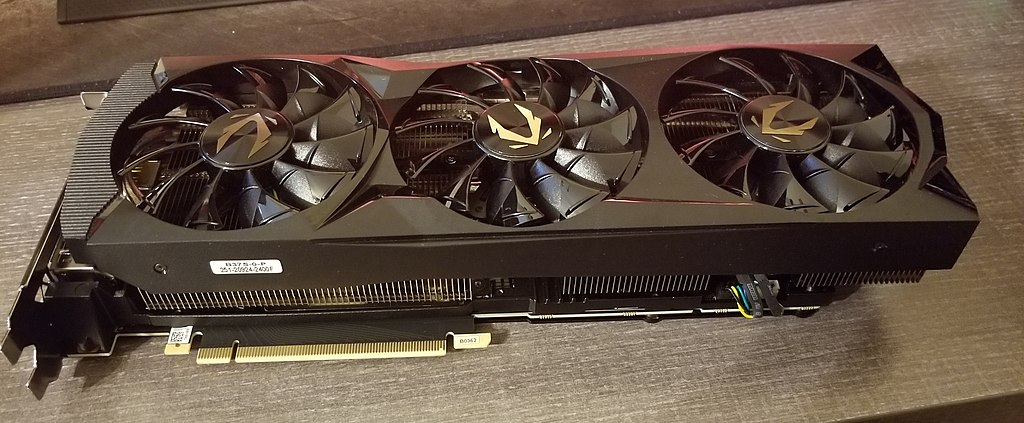
\includegraphics[width=\textwidth]{images/1024px-Zotac_Gaming_GTX_2080_ti.jpg}
    \caption{Beispiel einer Grafikkarte (Zotax Gaming 2080 ti) \cite{2080_ti_graphics_card}}
    \label{fig:2080_ti_graphics_card}
\end{figure}

\section{Rendering-Pipeline \cite[Vgl.][The Graphics Rendering Pipeline]{real_time_rendering}}
\label{sec:render_pipeline}
\begin{quote}
The main function of the [graphics rendering] pipeline is to generate, or \textit{render}, a two-dimensional image, given a virtual camera, three-dimensional objects, light sources, and more. The rendering pipeline is thus the underlying tool for real-time rendering.

-- Real-Time Rendering \cite[S. 11]{real_time_rendering}
\end{quote}

\subsection{Architektur}
Grundsätzlich besteht die Rendering-Pipeline aus vier Abschnitten, die mehr oder weniger frei programmierbar sind (siehe Abbildung \ref{fig:render_pipeline}). Generell läuft der Abschnitt \textit{Anwendung} auf der \ac{CPU} (kann aber auch teilweise mithilfe von \ac{GPU}-Compute auf der \ac{GPU} implementiert werden) und beschreibt die Logik der Anwendung. Die drei folgenden Abschnitte \textit{Geometrieverarbeitung}, \textit{Rasterung} und \textit{Pixelverarbeitung} laufen alle auf der \ac{GPU}, wobei die \textit{Geometrie-} und \textit{Pixelverarbeitung} hier frei mit \textit{Shadern} programmierbar sind und die \textit{Rasterung} nur über Parameter konfiguriert werden kann.

Ursprünglich wurde der Begriff \textit{Shader} für Programme benutzt, die zur Farb- und Helligkeitsbestimmung einer 3D-Szene beigetragen haben. Da diese Aufgaben sich dann als Spezialität der \ac{GPU} herausgestellt haben, wurde der Begriff \textit{Shader} immer weiter gefasst und bezeichnet heute grundsätzlich ein \ac{GPU}-Programm.

\begin{figure}
    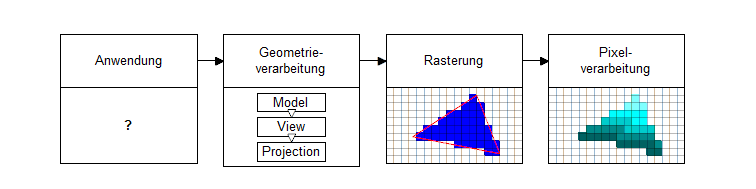
\includegraphics[width=\textwidth]{images/render_pipeline.png}
    \caption{Grundsätzlicher Aufbau der Rendering-Pipeline, unterteilt in die vier Abschnitte \textit{Anwendung}, \textit{Geometrieverarbeitung}, \textit{Rasterung} und \textit{Pixelverarbeitung}}
    \label{fig:render_pipeline}
\end{figure}

\subsection{Anwendung}
Der Abschnitt \textit{Anwendung} kann nicht konkret beschrieben werden, da er sich, wie der Name schon sagt, von Anwendung zu Anwendung unterscheidet. Jedoch kann man grundsätzlich sagen, dass hier die Logik der Anwendung stattfindet, wie zum Beispiel:
\begin{itemize}
\item{Benutzereingaben verarbeiten und auswerten}
\item{Physikberechnungen zwischen den Objekten}
\item{Ressourcen von der Festplatte laden}
\end{itemize}
Damit bereitet der Abschnitt \textit{Anwendung} die Daten für die restlichen Abschnitte vor und entscheidet, was dafür in Betrachtung gezogen wird (zum Beispiel nur Objekte in Blickrichtung der virtuellen Kamera).

\subsection{Geometrieverarbeitung}
\label{sub:geometry_processing}
Die \textit{Geometrieverarbeitung} ist dafür zuständig, die Geometriedaten (\textit{vertices} (Eckpunkte)) für die Rasterung vorzubereiten. Dafür müssen die \textit{vertices} meist zuerst von ihrer lokalen Position (innerhalb des Objektes) in die Position innerhalb des Sichtfeldes der virtuellen Kamera umgewandelt werden. 

\begin{figure}
    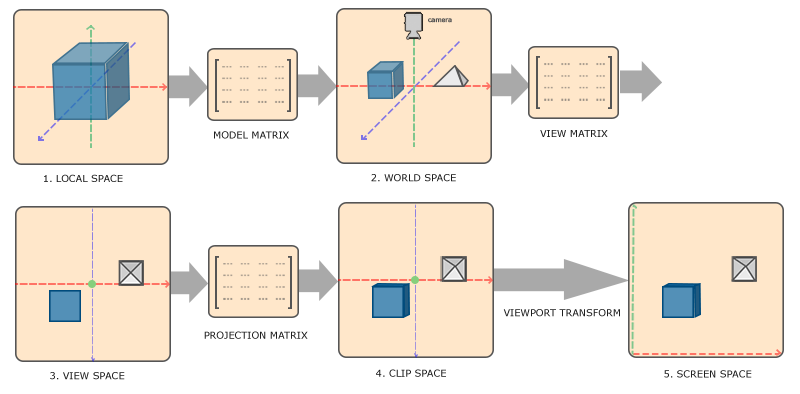
\includegraphics[width=\textwidth]{images/mvp_matrix.png}
    \caption{Transformation von Objekt bezogenen Vertexdaten in den \textit{world space}, dann in den \textit{view space} und schlussendlich in den \textit{clip space}. Die finale Umwandlung vom \textit{clip space} in den \textit{screen space} passiert dabei automatisch und verschiebt den Ursprung von der Mitte in entweder die ober oder untere (abhängig von der verwendeten Grafik-API) linke Ecke. \cite{learnopengl:coordinate_systems}}
    \label{fig:mvp_matrix}
\end{figure}

Dies passiert normalerweise mithilfe mehrerer Matrizen (siehe Abbildung \ref{fig:mvp_matrix}). Dabei wandelt die \textit{Model}-Matrix die lokalen Vertexdaten in das globale (\textit{world}) Koordinatensystem um. Die \textit{View}-Matrix wandelt dann die transformierten Daten wiederum in das lokale System der virtuellen Kamera um. Schlussendlich projiziert die \textit{Projection}-Matrix die Vertexdaten aus dem dreidimensionalen Raum auf die Bildebene. 

Die \textit{Model}-Matrix ist dabei abhängig von der Transformation des jeweiligen Objektes im \textit{world space}. Aus der Transformation der Kamera ergibt sich die \textit{View}-Matrix und die \textit{Projection}-Matrix wird aus den speziellen Eigenschaften der Kamera (Sichtfeld und \textit{near-}/\textit{far-plane} bei einer perspektivischen Projektion) gebildet. Manchmal werden die einzelnen Matrizen \textit{Model}, \textit{View} und \textit{Projection} auch zur sogenannten \textit{ModelViewProjection}-Matrix zusammengefasst um die Anzahl der Vektor-Matrix-Multiplikationen zu verringern.

Der Abschnitt Geometrieverarbeitung ist bis auf die finale Umwandlung vom \textit{clip space} in den \textit{screen space} frei programmierbar. Dabei wird ein zugewiesener Vertex-\textit{Shader} für jeden Vertex aufgerufen. Da dieser Abschnitt aber auf der \ac{GPU} läuft, kann man die Geometrieverarbeitung aber nicht mit einer üblichen Programmiersprache für \ac{CPU}s implementieren, sondern muss eine Programmiersprache für \textit{Shader}, wie zum Beispiel GLSL verwenden. Die Syntax von \ac{GLSL} ist dabei stark an der von C angelehnt. 

In Listing \ref{lst:vertex_shader} sieht man die Implementierung der Geometrieverarbeitung in der, bei dieser Arbeit entstandenen, \textbf{spider}-Engine. Dabei werden die Matrizen \textit{Model}, \textit{View} und \textit{Projection} einzeln dem Shader übergeben und sind für alle Shader-Ausführungen (für dieses Objekt) konstant. Jedoch unterscheiden sich bei jeder Ausführung die Daten des jeweiligen Vertex, für den der \textit{Shader }ausgeführt wird. Diese spezifischen Daten bekommt der Shader in den 4 Eingangsparametern ab Zeile 14 übergeben:
\begin{itemize}
\item{\textit{inPosition}: die Position des Vertex innerhalb des Objektes}
\item{\textit{inTexCoords}: die Texturkoordinaten des Vertex, zur späteren Bestimmung von Materialeigenschaften in der Pixelverarbeitung}
\item{\textit{inNormal}: die Normale des Vertex, meist aus den Normalen der angrenzenden Polygonflächen berechnet}
\item{\textit{inTangent}: die Tangente des Vertex, wird zur Anwendung von \textit{normal maps} in der Pixelverarbeitung benötigt}
\end{itemize}

Die 4 Ausgangsparameter ab Zeile 19 werden dann später, nach der Interpolation bei der Rasterung, in der Pixelverarbeitung benutzt. Wobei der Prefix \textit{frag} hier für \textit{fragment} steht, was eine alternative Bezeichnung für einen Pixel ist.
\begin{itemize}
\item{\textit{fragPosWorld}: die Position des Pixels im \textit{world space}}
\item{\textit{fragTexCoords}: die Texturkoordinaten des Pixels}
\item{\textit{fragNormal}: die Normale des Pixels}
\item{\textit{fragTangent}: die Tangente des Pixels}
\end{itemize}

\textit{gl\_Position} ist ein von \ac{GLSL} reservierter Ausgansparameter in dem die berechnete Vertexposition, zur weiteren Nutzung in folgenden Pipeline-Abschnitten, im \textit{clip space} gespeichert werden soll. Die lokale Vertexposition wird dabei zuerst vom lokalen System des Objektes mithilfe der \textit{Model}-Matrix in den \textit{world space} transformiert.  Diese Position wird dann einerseits direkt in \textit{fragPosWorld} abgespeichert und anderseits mithilfe der \textit{View}- und \textit{Projection}-Matrizen in den \textit{clip space} transformiert und in \textit{gl\_Position} gespeichert. Der Wert für \textit{fragTexCoords} wird direkt von \textit{inTexCoords} übernommen, da er unabhängig vom jeweiligen Koordinatensystem ist. Da \textit{inNormal} und \textit{inTangent} jeweils normalisierte Vektoren (also Richtungen) darstellen, können diese nicht mit der normalen \textit{Model}-Matrix in den \textit{world space} transformiert werden. Dazu muss erst die Transponierte der inversen \textit{Model}-Matrix gebildet werden. Mit dieser können dann \textit{fragNormal} und \textit{fragTangent} jeweils von \textit{inNormal} und \textit{inTangent} berechnet werden.

\begin{minipage}{\textwidth}
\begin{lstlisting}[language=GLSL, label={lst:vertex_shader}, caption={Beispiel eines Vertex Shaders in \ac{GLSL}, welcher so in der \textbf{spider}-Engine verwendet wird}]
#version 450
#extension GL_ARB_separate_shader_objects : enable

layout(set = 0, binding = 0) uniform Model {
    mat4 model;
};

layout(set = 0, binding = 1) uniform Camera {
    mat4 view;
    mat4 proj;
    vec3 pos;
} cam;

layout(location = 0) in vec3 inPosition;
layout(location = 1) in vec2 inTexCoords;
layout(location = 2) in vec3 inNormal;
layout(location = 3) in vec3 inTangent;

layout(location = 0) out vec3 fragPosWorld;
layout(location = 1) out vec2 fragTexCoords;
layout(location = 2) out vec3 fragNormal;
layout(location = 3) out vec3 fragTangent;

void main() {
    vec3 pos_world = vec3(model * vec4(inPosition, 1.0));
    gl_Position = cam.proj * cam.view * vec4(pos_world, 1.0);
    fragPosWorld = pos_world;
    fragTexCoords = inTexCoords;
    mat3 to_world = mat3(transpose(inverse(model)));
    fragNormal = to_world * inNormal;
    fragTangent = to_world * inTangent;
}
\end{lstlisting}
\end{minipage}
\subsection{Rasterung}
\label{sub:rasterizing}
Nach der \textit{Geometrieverarbeitung} sind nun alle Vertices des Polygons (im Folgenden zur Vereinfachung als Beispiel ein Dreieck) in den \textit{screen space} transformiert worden. Falls die Vertices im Bild liegen, d.h sie haben sowohl im vertikalen, als auch horizontalen Bereich des \textit{screen space} Werte zwischen 0 und 1, müssen nun die Pixel bestimmt werden, die in dem Dreieck liegen. Bei Polygonen die teilweise innerhalb und teilweise außerhalb des sichtbaren Bereichs liegen, wird das Polygon automatisch so zerstückelt, dass nur die sichtbaren Teile berücksichtigt werden (siehe Abbildung \ref{fig:screen_space}).

\begin{figure}
    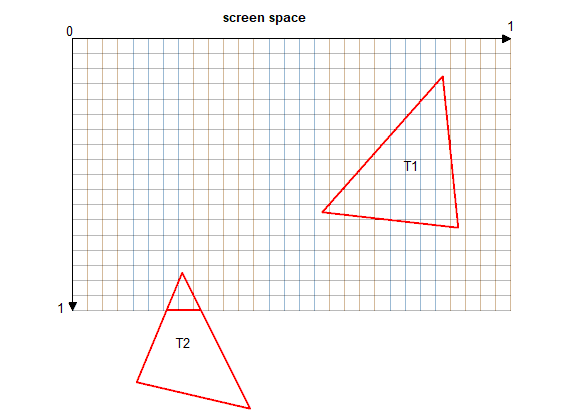
\includegraphics[width=\textwidth]{images/screen_space_rasterizing.png}
    \caption{Zwei Dreiecke \textbf{T1} und \textbf{T2} im \textit{screen space}. \textbf{T1} wird hierbei komplett gerastert und \textbf{T2} erst so zerteilt, dass nur der sichtbare Bereich gerastert werden muss.}
    \label{fig:screen_space}
\end{figure}

Die \textit{Rasterung} ist hierbei fest in der Hardware einer \ac{GPU} verbaut und kann nur per Parameter konfiguriert werden. Dazu zählen zum Beispiel:

\begin{itemize}
\item{Art der zu rasternden Primitive: Punkte, Linien oder Dreiecke}
\item{Wie soll die Vorderseite eines Dreiecks bestimmt werden? Vertices sind entweder im oder gegen den Uhrzeigersinn angeordnet}
\item{Welche Seiten eines Dreieckes sollen berücksichtigt werden? Nur die Vorderseite, nur die Rückseite oder beide?}
\end{itemize}

Nun wird für jeden Pixel, der im Polygon liegt, die Vertexeigenschaften, d.h. die Ausgansparameter der Geometrieverarbeitung, zwischen den Vertices des Polygons interpoliert (siehe Abbildung \ref{fig:barycentric_color}). Für jeden dieser Pixel wird dann mit den interpolierten Eigenschaften als Eingangsparameter der \textit{Pixel-Shader}, oder auch \textit{Fragment-Shader}, zum finalen Abschnitt der Pixelverarbeitung aufgerufen. 

\begin{figure}
    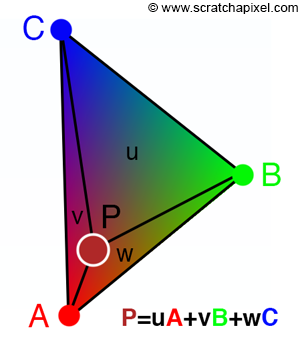
\includegraphics[scale=1]{images/barycentriccolor.png}
    \caption{Interpolation von Vertexdaten innerhalb eines Dreiecks am Beispiel der Farbinformation der Vertices mithilfe von baryzentrischen Koordinaten \cite{scratchapixel:barycentric_color}}
    \label{fig:barycentric_color}
\end{figure}

\subsection{Pixelverarbeitung}
In der \textit{Pixelverarbeitung} wird der finale Farbwert eines Pixels berechnet im \textit{Framebuffer} gespeichert. Der \textit{Framebuffer} besteht dabei aus einem (oder auch mehreren) \textit{color buffer}, was im Prinzip ein zwei dimensionales Array (in Größe der Pixelanzahl: Breite * Höhe) für Farbwerte ist. Dazu kommt ein gleich großer \textit{depth buffer} der für jeden Pixel einen Tiefenwert (Distanz zur Kamera) abspeichert. Mit dem \textit{depth buffer} kann somit pro Pixel verglichen werden, ob der aktuell zu bearbeitende Punkt näher an der Kamera (Farbwert des Punktes wird berechnet und überschreibt den Tiefenwert) oder weiter weg ist (Punkt wird nicht weiter beachtet).

Der \textit{depth buffer} bietet hierbei den Vorteil, dass die Polygone nicht von \quotize{hinten (fern) nach vorne (nah)} gezeichnet werden müssen. Dadurch, dass jeder Punkt nur mit dem aktuell der Kamera am nächsten verglichen werden muss, können die Polygone in beliebiger Reihenfolge bearbeitet werden. Dies gilt allerdings nur für opake, nicht transparente, Objekte. Bei teil-transparenten Objekte muss trotzdem noch auf die Zeichenreihenfolge geachtet werden.

Falls der gerasterte Pixel erfolgreich mit dem aktuellen Tiefenwert verglichen wurde, d.h. er ist näher an der Kamera wird für ihn der \textit{Pixel-Shader}, im folgenden als \textit{Fragment-Shader} bezeichnet, aufgerufen. Als Beispiel kann hier der \textit{Fragment-Shader} für \ac{PBR} in der \textbf{spider}-Engine gesehen werden (siehe Anhang \ref{appendix:b}). Der  \textit{Fragment-Shader} berechnet dabei aus den interpolierten Vertexdaten und anderen Eingaben (zum Beispiel zusätzliche Daten wie Texturen) einen Farb- und Transparenzwert. Auch kann hier der Pixel noch verworfen werden, wenn zum Beispiel ein Transparenzwert von \textbf{0} (voll-transparent) berechnet wurde.

Die Pixelverarbeitung kann man also wiederum in drei Teilabschnitte unterteilen: 
\begin{itemize}
\item[1)]{Vergleichen mit dem aktuellen Tiefenwert aus dem \textit{depth buffer}}
\item[2)]{Berechnen des Farbwertes}
\item[3)]{Zusammenfügen mit dem aktuell im \textit{color buffer} gespeicherten Farbwert}
\end{itemize} 
Dabei ist hier nur der Teilabschnitt 2) frei per \textit{Shader} programmierbar. Teilabschnitte 1) und 3) können ähnlich wie im Abschnitt Rasterung (\ref{sub:rasterizing}) mit Parametern konfiguriert werden.

\section{Grafik-APIs \cite[Vgl.][The Evolution of Programmable Shading and APIs]{real_time_rendering}}
\textit{Der Begriff \quotize{\ac{GPU}} wurde erstmals 1999 von NVIDIA eingeführt, jedoch werden im folgenden der Einfachheit halber alle vorherigen Chips mit ähnlicher Funktion unter dem Begriff \quotize{\ac{GPU}} zusammengefasst.}

\begin{figure}
    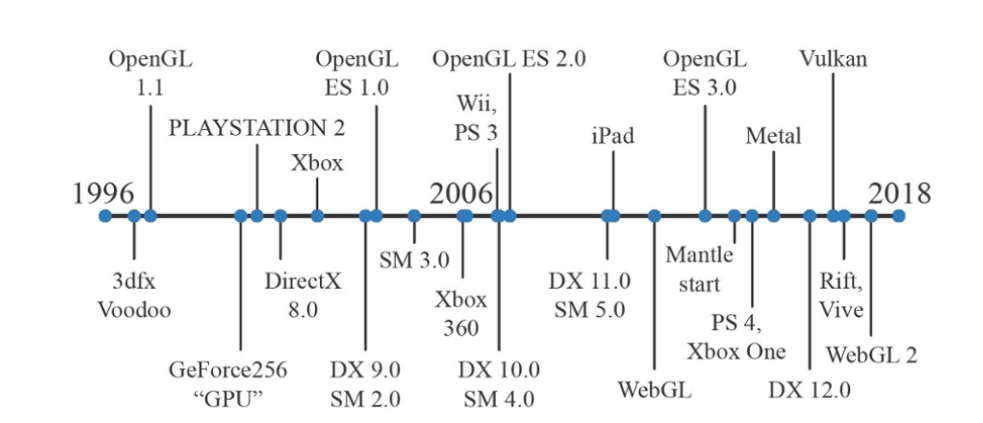
\includegraphics[width=\textwidth]{images/api_timeline.png}
    \caption{Zeitlinie mit wichtigen Grafik-API- und Hardwareerscheinungen \cite[S. 38]{real_time_rendering}}
    \label{fig:barycentric_color}
\end{figure}

Analog zu den Programmiersprachen für \ac{CPU}s, wurden auch Ideen zur Programmierung von \ac{GPU}s, entwickelt bevor es die Hardware unterstützt hat. So wurden frei programmierbare \textit{Shader} wurde erstmals in Cooks \textit{Shade Trees} \cite{cook:shade_trees} erwähnt. Daraufhin wurde in den späten 1980er Jahren die RenderMan Shading Language \cite{pixar:rsl} entwickelt, welche auch heute noch in der Filmproduktion eingesetzt wird. Zu diesem Zeitpunkt waren \ac{GPU}s aber nichts weiter wie fest in die Hardware implementierte Bildspeicher mit einfachsten Funktionen \cite[Vgl.][]{gpu_history}.

Die erste \ac{GPU} zur Beschleunigung von 3D-Szenen, die 3dfx Voodoo \cite{wikipedia:3dfx_voodoo}, hatte die Rendering-Pipeline direkt in die Hardware implementiert. Auch die NVIDIA GeForce 256 \cite{wikipedia:geforce256}, die erste \ac{GPU}, die auch tatsächlich so bezeichnet wurde, konnte nicht programmiert werden. Dafür konnte die integrierte Rendering-Pipeline zumindest konfiguriert werden.

Im Jahre 2001 ist mit der NVIDIA Geforce 3 \cite{wikipedia:geforce3} die erste teilweise programmierbare \ac{GPU} erschienen. Durch die Grafik-APIs Microsoft DirectX 8.0 und das nicht-proprietäre OpenGL konnte hier die \textit{Vertex-Shader} mit einer Assembly-artigen Sprache programmiert werden. Mit DirectX 8.0 wurde auch das Konzept des \textit{Shader Model (SM)} \cite[Vgl.][Shader model comparison]{wikipedia:hlsl} eingeführt, welches spezifiziert welche Eigenschaften (zum Beispiel, wie viele Register dem Shader-Programm zur Verfügung stehen), die jeweilige Hardware erfüllen muss. Zwar unterstütze DirectX 8.0 auch programmierbare \textit{Pixel-Shader} (in OpenGL \textit{Fragment-Shader} genannt), jedoch waren diese noch sehr eingeschränkt im Funktionsumfang.

Dabei funktionieren \ac{GPU}s bis heute so, dass das gleiche Shader-Programm gleichzeitig auf mehrere Eingabedaten mit der selben Struktur, zum Beispiel Vertexdaten bei einem \textit{Vertex-Shader}, angewandt wird. Dadurch konnten in den Shader-Programmen für die ersten \ac{GPU}s noch keine Verzweigungen benutzt werden, da diese ja potentiell zu unterschiedliche Anweisungen für die jeweiligen Daten führen. Dies wurde von Shader-Programmierern dadurch umgangen, dass einfach alle Anweisungen aller potentiellen Verzweigungen nacheinander ausgeführt wurden und danach die nicht gebrauchten Ergebnisse verworfen wurden. Das führte zwar zu \quotize{nutzlosen} Berechnungen, jedoch war dies durch die Parallelität insgesamt immer noch schneller, als die Daten sequentiell zu verarbeiten.

Mit dem Erscheinen von DirectX 9.0 mit Shader Model 2.0 im Jahre 2002, hatten Programmierer endlich die volle Kontrolle über sowohl \textit{Vertex-} als auch \textit{Fragment-Shader}. Für den offenen Standard OpenGL wurde diese Möglichkeit relativ zeitgleich durch \textit{extensions} ermöglicht. Außerdem konnten die Shader nun in einer C ähnlichen Sprache geschrieben werden: \ac{HLSL} \cite{wikipedia:hlsl} für DirectX und \ac{GLSL} \cite{wikipedia:hlsl} für OpenGL. Mit der Einführung des Shader Model 3.0 im Jahre 2004 konnte nun endlich auch ein dynamischer Programmablauf mit Verzweigungen im Shader benutzt werden. Mit der Einführung der Spielekonsole Nintendo Wii Ende 2006 wurde auch eine der letzten \ac{GPU}s mit fester Rendering-Pipeline eingeführt. 

Ebenfalls wurde Ende 2006 DirectX 10.0 und Shader Model 4.0 eingeführt, welche eine neue Art von Shadern (\textit{Geometry-Shader}) und die Vereinheitlichung des Shader-Designs mit sich brachte. Mit DirectX 11.0 und Shader Model 5.0 im Jahre 2009 wurden schließlich unter anderem \textit{Compute-Shader} eingeführt. Die Version von OpenGL mit ähnlichem Funktionsumfang ist dabei 4.3.

Bis dahin war das Paradigma für Grafik-APIs dem Entwickler so viel Arbeit wie möglich abzunehmen und zum Beispiel im Treiber Eingaben zu validieren und Ressourcen (zum Beispiel Texturen und Buffer) automatisch zu verwalten. Dies änderte sich 2013 mit der Einführung von Mantle durch den \ac{CPU}- und \ac{GPU}- Hersteller \ac{AMD} als Alternative zu Direct3D und OpenGL. Die Idee hinter der API, die in Zusammenarbeit mit dem Videospielentwickler DICE entwickelt wurde, war es, den Overhead im Grafiktreiber so viel wie möglich zu reduzieren und diese Kontrolle dem Entwickler zurückzugeben. Microsoft hat die Ideen hinter Mantle aufgenommen und 2015 mit DirectX 12.0 eine DirectX Version dieses neuen Paradigmas veröffentlicht. Wichtig ist hier, dass DirectX 12 keinen Fokus auf neuen Funktionen hat, sondern nur die Verwendung der API radikal geändert hat. Bei der Einführung von DirectX 12.0 hatte es die gleichen Funktionalitäten wie das damals aktuelle DirectX 11.3. Auch Apple hat 2014 mit Metal ihre eigene \quotize{low-overhead} API veröffentlicht. Diese debütierte zuerst auf den mobilen Geräten wie iPhone und iPad, war jedoch ein Jahr später auch auf Macs verfügbar. Währenddessen hatte AMD ihre Arbeit zu Mantle an das für OpenGL zuständige Konsortium Khronos Group gestiftet. Diese führte 2016 mit Vulkan ihre Version einer \quotize{low-overhead} API ein. Ähnlich wie bei den DirectX-Versionen 11 und 12, hat Vulkan hier OpenGL nicht abgelöst, sondern stellt nur eine Alternative dar. Mit Vulkan wurde auch eine Zwischensprache (engl. \textit{intermediate language}) für Shader-Programme, ähnlich wie LLVM IR, mit dem Namen SPIR-V eingeführt, die es dem Entwickler erlaubt Shader vor zu kompilieren.

Für mobile Geräte gibt es OpenGL ES (\quotize{Embedded Systems}) welches 2003 als eine im Funktionsumfang verringerte Version von OpenGL 1.3 veröffentlicht wurde. OpenGL ES 1.0 beschrieb noch eine feste Rendering-Pipeline, welche aber durch Version 2.0 im Jahr 2007 die Möglichkeiten zur Shader-Programmierung erhielt. OpenGL ES 3.0 wurde schließlich 2012 eingeführt und brachte viele bekannte Funktionen der \quotize{großen Brüder} OpenGL und DirectX mit.

Die Grafik-API für Webbrowser WebGL basiert wiederum auf OpenGL ES, wurde 2011 veröffentlicht und ist mit Version 2.0 von OpenGL ES im Funktionsumfang äquivalent. WebGL 2.0 wurde 2017 eingeführt und nutzt OpenGL ES 3.0.


\chapter{WebGPU}
\label{cha:webgpu}

\section{Entstehung \cite[Vgl.][]{wikipedia:webgpu}}
Da WebGL auf dem alten API-Paradigma von OpenGL und DirectX vor Version 12 beruht, wurden Rufe laut, dass es auch eine \quotize{moderne} Grafik-API für Webbrowser geben sollte, um deren Vorteile auch im Web nutzen zu können.

Die ersten Vorstöße dazu gab es als Google Mitarbeiter bei einer Präsentation Mitte 2016 für die WebGL Arbeitsgruppe über die grundlegenden Ideen und Prinzipien für eine moderne Grafik-API fürs Web, damals noch als \quotize{WebGL Next} bezeichnet, sprachen. Diese Ideen wurden dann Anfang 2017 von der Khronos Group aufgegriffen und in einem Meeting hat ein Google Team dann ihren mit \quotize{NXT} betitelten Prototypen präsentiert, welcher im Webbrowser Chromium lief und sich an Konzepten von Vulkan, DirectX 12 und Metal bediente. Teams von Apple und Mozilla hatten außerdem Prototypen für Safari und Servo (die Browser Engine für Firefox) gebaut, welche sich an Apples Metal API orientiert haben. 

Kurze Zeit später wurde die W3C Gruppe \quotize{GPU for the Web} gegründet und \quotize{WebGPU} als Arbeitstitel für die neue API beschlossen \cite{golem:webgpu}. Nachdem die meisten oberflächlichen Probleme im Standardisierungsprozess Mitte 2018 gelöst waren, gab Googles Chrome Team bekannt, dass sie den zukünftigen \textbf{WebGPU} in ihren Webbrowser implementieren möchten.

\section{Beschreibung}
\begin{minipage} {\textwidth}
\begin{quote}
\quotize{The mission of the GPU on the Web Community Group is to provide an interface between the Web Platform and modern 3D graphics and computation capabilities present in native system platforms. The goal is to design a new Web API that exposes these modern technologies in a performant, powerful and safe manner. It should work with existing platform APIs such as Direct3D 12 from Microsoft, Metal from Apple, and Vulkan from the Khronos Group. This API will also expose the generic computational facilities available in today's GPUs to the Web, and investigate shader languages to produce a cross-platform solution.}

-- GPU for the Web Community Group \cite{w3:community_gpu}
\end{quote}
\end{minipage}

\textbf{WebGPU} soll hierbei ähnlich wie bei Vulkan und OpenGL, und DirectX 12 und 11 nicht WebGL direkt ablösen, sondern erstmal nur eine Alternative bilden.

\section{WGSL}
\subsection{Übersicht}
Mit WGSL \cite{w3:wgsl} soll auch \textbf{WebGPU} eine eigene Shader-Sprache bekommen. Bisherige \textbf{WebGPU}-Implementierungen unterstützen jedoch bisher nur SPIR-V als Shader-Code. Dadurch konnte der Verfasser leider keine praktischen Erfahrungen bei der Verwendung von WGSL machen. Die \textbf{spider}-Engine, die diese Arbeit begleitet hat, verwendet daher GLSL-Shader, die zu SPIR-V kompiliert werden. Trotzdem werden im Folgenden die Grundprinzipien und Beispiele zu WGSL besprochen, da es in Zukunft wohl ein wichtiger Bestandteil von \textbf{WebGPU} sein wird. Jedoch ist hier zu beachten, dass dies nur dem aktuellen Stand der Spezifikation entspricht und sich hier noch vieles verändern kann.

\subsection{Kritik an WGSL}
\begin{minipage}{\textwidth}
\begin{lstlisting}[language=GLSL, label={lst:loop}, caption={for-Schleifen in GLSL und WGSL}]
// for-loop in GLSL
int a = 2;
const int step = 1;
for (int i = 0; i < 4; i += step) {
  if (i % 2 == 0) continue;
  a *= 2;
}

// "for-loop" in WGSL
const a : i32 = 2;
var i : i32 = 0;
loop {
  if (i >= 4) { break; }

  const step : i32 = 1;

  if (i % 2 == 0) { continue; }

  a = a * 2;

  continuing {
    i = i + step;
  }
}
\end{lstlisting}
\end{minipage}

WGSL soll \quotize{trivial von und zu SPIR-V konvertierbar} \cite[Vgl.][Goals]{w3:wgsl} sein, was unter anderem die Frage aufwirft, warum dann WGSL überhaupt benötigt wird \cite[Vgl.][]{github:wgsl_terrible}. Durch die Nähe zu der Zwischensprache SPIR-V ist die Syntax von WGSL für Entwickler, die mit einer bisherigen Shader-Sprache vertraut sind, nicht sehr üblich. Auch gibt es nicht die aus den meisten Programmiersprachen bekannten Schleifenstrukturen, sondern nur eine \texttt{loop}-Anweisung (siehe Listing \ref{lst:loop}), aber nicht direkt \texttt{for}, \texttt{while} oder \texttt{do-while} \cite[Vgl.][]{github:wgsl_loop}. In Zukunft soll nur noch WGSL als Shader-Sprache akzeptiert werden. Dazu müssten die bei vielen Entwicklern schon bestehenden GLSL- oder HLSL-Shader erst konvertiert werden. Dies würde in etwas so aussehen:

\texttt{GLSL/HLSL -> SPIR-V -> WGSL -> *WebGPU* -> SPIR-V/DXIL/MSL}

Für die Umwandlung von GLSL/HLSL zu SPIR-V gibt es bereits zahlreiche Tools, welche produktiv getestet und eingesetzt wurden, wie zum Beispiel, das in diesem Projekt genutzte \textit{glslc}, welches in der Shader-Werkzeugsammlung \textit{shaderc} \cite{shaderc} enthalten ist. Der abschließende Schritt, bei dem \textbf{WebGPU} den WGSL-Shader-Code wieder in \texttt{SPIR-V/DXIL/MSL} umwandeln muss, ist nötig, da WebGPU auf den jeweiligen nativen Grafik-APIs (Vulkan, DirectX 12, Metal) aufbaut, welche keinen WGSL-Shader-Code nutzen können.

Die Ursache für die Entscheidung für WGSL und gegen SPIR-V als primäres Shader-Code-Format, liegt wohl einerseits an der für das Web übliche Praxis, von Menschen lesbare Datenformate zu verwenden (kein Binärcode). Anderseits scheint es wohl rechtliche Spannungen zwischen Apple und der für SPIR-V verantwortlichen Khronos Group zu geben \cite[Vgl.][]{hacker_news:apple_khronos}.

\subsection{Vergleich zu GLSL und HLSL}
In diesem Abschnitt sollen die Grundlagen von WGSL aufgezeigt werden, im Besonderen im Bezug auf Unterschiede zu GLSL und HLSL. Da sich die Spezifikation von WGSL jedoch noch in Arbeit befindet, ist alles folgende nur auf Grundlage der zur Zeit des Verfassens dieses Abschnittes (24. Juni 2020) aktuellen Spezifikation.

\subsubsection{Skalare Typen}
\label{sub:scalars}
\begin{table}[htb]
\begin{center}
\begin{tabular}{ |l|l|l|l| }
    \hline
    \textbf{Typ} & \textbf{Beschreibung} & \textbf{GLSL} & \textbf{HLSL} \\
    \hline
    \multicolumn{4}{|l|}{Boolean} \\
    \hline
    \texttt{bool} & Entweder \texttt{true} oder \texttt{false} & \texttt{bool} & \texttt{bool} \\
    \hline
    \multicolumn{4}{|l|}{Numerisch} \\
    \hline
    \texttt{i32} & 32-bit Integer mit Vorzeichen & \texttt{int} & \texttt{int} \\
    \hline
    \texttt{u32} & 32-bit Integer ohne Vorzeichen & \texttt{uint} & \texttt{uint} \\
    \hline
    \texttt{f32} & 32-bit Fließkommazahl nach IEEE 754 & \texttt{float} & \texttt{float} \\
    \hline
    \textit{-} & 64-bit Fließkommazahl nach IEEE 754 & \texttt{double} & \texttt{double} \\
    \hline
\end{tabular}
\end{center}
\caption{Skalare Typen in WGSL mit den äquivalenten Typen in GLSL und HLSL}
\label{tab:scalars}
\end{table}

\subsubsection{Mehrkomponenten Typen}
\paragraph{Vektortypen} \

Vektortypen werden in WGSL mit 

\texttt{vec\textit{N}<\textit{T}>}

deklariert, wobei \textit{N} für die Anzahl der Komponenten und \textit{T} für den Datentyp steht. \textit{N} muss dabei in \{2, 3, 4\} und \textit{T} muss einer der skalaren Typen aus Abschnitt \ref{sub:scalars} sein.

Das äquivalente Gegenstück hierzu in GLSL wäre 

\texttt{\textit{T}vec\textit{N}}

wobei \textit{T} hier als Abkürzung eines skalaren Typen fungiert (b = \texttt{bool}, i = \texttt{int}, u = \texttt{uint}, d = \texttt{double}). Wenn \textit{T} weggelassen wird, wird der skalare Typ \texttt{float} verwendet, da dies der mit Abstand meist verwendete skalare Typ in der Shader-Programmierung ist. \textit{N} muss hier ebenfalls in \{2, 3, 4\} sein.

Bei HLSL werden Vektortypen wie folgt deklariert:

\texttt{\textit{T}\texttt{N}}

Wobei \textit{T} hier einer der skalaren Typen sein muss und \textit{N} entweder in \{1, 2, 3, 4\} oder gar nicht vorkommen darf. Das Weglassen von \textit{N} oder N = 1 resultieren beide in dem skalaren Typen \textit{T}.

So würde ein 3-komponentiger Vektor vom Typ \texttt{f32} bzw. \texttt{float} in den jeweiligen Sprachen so aussehen:
\begin{itemize}
 \item WGSL: \texttt{vec3<f32>}
 \item GLSL: \texttt{vec3}
 \item HLSL: \texttt{float3}
\end{itemize}

\paragraph{Matrixtypen} \

Analog zu Vektortypen werden Matrixtypen in WGSL mit

\texttt{mat\textit{N}x\textit{M}<\textit{T}>}

deklariert, wobei \textit{N} hier für die Anzahl der Spalten und \textit{M} für die Anzahl der Zeilen steht. \textit{N} und \textit{M} müssen wiederum beide in \{2, 3, 4\} sein. \textit{T} ist ein skalarer Typ aus Abschnitt \ref{sub:scalars}.

In GLSL gibt es dafür

\texttt{mat\textit{N}x\textit{M}}

und als Abkürzung für eine Matrix mit quadratischer Form (Anzahl Spalten = Anzahl Zeilen)

\texttt{mat\textit{N}}

Matrixkomponenten sind immer vom Typ \texttt{float} oder \texttt{double}. Eine Matrix mit doppelter Genauigkeit wird mit \texttt{dmat\textit{N}x\textit{M}} bzw \texttt{dmat\textit{N}} deklariert.

In HLSL werden die Matrixtypen ähnlich wie die Vektortypen deklariert:

\texttt{\textit{T}\texttt{N}x\texttt{M}}

wobei hier wie bei GLSL für \textit{T} jeder der skalare Typen benutzt werden kann. \textit{N} steht für die Anzahl der Spalten und \textit{M} für die Anzahl der Zeilen und beide müssen jeweils in \{1, 2, 3, 4\} sein.

Eine quadratische Matrix mit 3 Spalten und 3 Zeilen vom Typ \texttt{f32} bzw. \texttt{float} wird also jeweils so erstellt:
\begin{itemize}
 \item WGSL: \texttt{mat3x3<f32>}
 \item GLSL: \texttt{mat3x3} bzw. \texttt{mat3}
 \item HLSL: \texttt{float3x3}
\end{itemize}

Um wiederum eine Matrix mit 3 Spalten und 2 Zeilen vom Typ \texttt{i32} bzw. \texttt{int} zu erstellen werden folgende Deklarationen benötigt:

\begin{itemize}
 \item WGSL: \texttt{mat3x2<i32>}
 \item GLSL: \textit{-}
 \item HLSL: \texttt{int3x2}
\end{itemize}

\paragraph{Swizzling} \

Um auf die Komponenten eines Mehrkomponenten Typen zuzugreifen haben diese vordefinierte Felder. So hat ein 4-komponentiger Vektor zum Beispiel die Felder \texttt{x, y, z, w}. Da aber 4-komponentige Vektor auch häufig für Farbwerte benutzt werden, gibt es zusätzlich noch die Felder \texttt{r, g, b, a}, wobei dies aber nur andere Namen für die gleichen Komponenten sind: \texttt{x = r, y = g, z = b, w = a}. GLSL hat zusätzlich noch das Namensset \texttt{s, t, p, q}, das im Zusammenhang mit Texturkoordinaten benutzt wird.

Eine Besonderheit in vielen Shader-Sprachen ist es, dass diese Felder frei kombiniert werden können um die einzelnen Komponenten umzustrukturieren, was \textit{swizzling} \cite{wikipedia:swizzling} genannt wird (siehe Listing \ref{lst:swizzling}).

\begin{minipage}{\textwidth}
\begin{lstlisting}[language=GLSL, label={lst:swizzling}, caption={\quotize{Swizzling} von Komponenten in GLSL}]
vec4 some_vec = vec4(1.0, 2.0, 3.0, 4.0);
// Get the second component
float val = some_vec.y;
// Get the fourth as the first, and the first as the second component of a new vec2
vec2 other_vec = some_vec.ar; 
// Write to the first, third and second component
some_vec.xzy = vec3(0.0, some_vec.xx);
// But you can't mix name sets
vec3 faulty_vec = some_vec.xrr;
\end{lstlisting}
\end{minipage}

Dabei wird es in WGSL nicht möglich sein, in mehrere Komponenten gleichzeitig zu schreiben, also einen \quotize{swizzled} Ausdruck auf der linken Seite einer Zuweisung zu haben \cite[Vgl.][Typed Storage]{w3:wgsl}.

\subsubsection{Variablen} \

Im Gegensatz zu den C ähnlichen Sprachen GLSL und HLSL, verwendet WGSL eine Syntax zur Variablendefinition, die häufig in \quotize{moderneren} Sprachen wie Rust oder TypeScript benutzt wird:

\texttt{var \textit{Name} : \textit{Type} \textit{[= InitialValue]};} 

bzw. 

\texttt{const \textit{Name} : \textit{Type} = \textit{Value};}

Wird der initiale Wert weggelassen, wird die Variable mit  \texttt{0} (bzw. \texttt{0.0} / \texttt{false}) initialisiert \cite[Vgl.][Zero values]{w3:wgsl}.

\subsubsection{Strukturen} \

Eine Struktur ist ein Tupel mit \textit{N} Felder, wobei \textit{N} eine Ganzzahl größer \texttt{0} ist. Die Felder \textit{T1} bis \textit{TN} haben jeweils einen Datentyp, welcher wiederum eine Struktur sein kann (siehe Listing \ref{lst:wgsl_structs}).

\begin{minipage}{\textwidth}
\begin{lstlisting}[language=GLSL, label={lst:wgsl_structs}, caption={Definition und Benutzung von Strukturen in WGSL}]
type Student = struct {
  grade : i32;
  GPA : f32;
  attendance : array<bool,4>;
};

# The zero value for Student
var student: Student = Student(2, 1.5, array<bool,4>(false,false,true,false));
\end{lstlisting}
\end{minipage}

\section{Der aktuelle Stand}
\subsection{Spezifikation}
\textit{Unter \url{https://gpuweb.github.io/gpuweb/} \cite{w3:webgpu} kann die aktuellste Version der Spezifikation eingesehen werden.}

Zum Zeitpunkt des Verfassens dieses Abschnittes (24. Juni 2020) steht ein Großteil der \textbf{WebGPU}-Spezifikation fest. Jedoch gibt es noch immer Punkte bei denen noch keine Einigung gefunden werden konnte. Da der Großteil der Implementierung der \textbf{spider}-Engine vor Juni 2020 statt gefunden hat, werden die folgenden Beschreibungen und Erkenntnisse zur Zeit der Abgabe der Arbeit (oder insbesondere zu einem späteren Zeitpunkt) nicht mehr zwingend aktuell sein. An der grundlegenden Struktur oder den grundlegenden Mechaniken zur Verwendung von \textbf{WebGPU} sollte sich zwar nicht mehr allzu viel ändern, trotzdem sollte die folgenden Abschnitte nicht als direkte Vorlage zum Implementieren einer \textbf{WebGPU}-Applikation gesehen wird.



\subsection{Aktuelle Unterstützung in Webbrowsern}
\textit{Der aktuelle Stand der Implementierung in Webbrowsern kann unter \url{https://github.com/gpuweb/gpuweb/wiki/Implementation-Status} \cite{webgpu:implementation_status} eingesehen werden.}

Der produktive Nutzen von \textbf{WebGPU} hängt in erster Linie von der Unterstützung in den Webbrowsern ab. Laut StatCounter \cite{statcounter:browser} benutzten im Mai 2020 über 95\% aller Nutzer einer der in Tabelle \ref{tab:browser_share} aufgelisteten Webbrowser.

\begin{table}[htb]
\begin{center}
\begin{tabular} { |l|r| }
  \hline
  \textbf{Webbrowser} & \textbf{Marktanteil} \\
  \hline
  Chrome & 63,93\% \\
  \hline
  Safari & 18,19\% \\
  \hline
  Firefox & 4,38\% \\
  \hline
  Samsung Internet & 3,28\%\\
  \hline
  Edge Legacy & 2,13\%\\
  \hline
  UC Browser & 2,00\% \\
  \hline
  Opera & 1,92\% \\
  \hline
  Internet Explorer & 1,40\% \\
  \hline
\end{tabular}
\end{center}
\caption{Marktanteile der verbreitetsten Webbrowser im Mai 2020 laut StatCounter \cite{statcounter:browser}}
\label{tab:browser_share}
\end{table}

Wobei hier anzumerken ist, dass sowohl Chrome \cite{wikipedia:google_chrome}, Samsung Internet \cite{wikipedia:samsung_internet} und Opera \cite{wikipedia:opera} auf dem Webbrowser Chromium basieren. Chromium, Safari und Firefox haben jeweils eine experimentelle \textbf{WebGPU}-Implementierung, jedoch nur in den jeweiligen Preview-Versionen der Webbrowser. Dies lässt jedoch trotzdem den Schluss zu, dass \textbf{WebGPU} für mindestens 90\% der Nutzer in naher Zukunft zur Verfügung stehen wird.

\subsubsection{Chromium \cite{chromium} / Dawn \cite{google:dawn}}
\textit{Dawn} ist eine Open-Source \textbf{WebGPU}-Implementierung, die in dem Open-Source Webbrowser Chromium verwendet wird. 

Die \quotize{native} Implementierung von \textit{Dawn} benutzt dafür die Grafik-APIs der jeweils ausführenden Plattform:

\begin{itemize}
\item{\textit{D3D12} auf Windows 10}
\item{\textit{Metal} auf macOS und iOS}
\item{\textit{Vulkan} auf Windows, Linux und Google eigenen Betriebssystemen (ChromeOS, Android, Fuchsia)}
\item{\textit{OpenGL} wo verfügbar}
\end{itemize}

Das heißt, dass die \textbf{WebGPU}-Befehle hier im Hintergrund die jeweiligen Befehle der nativen Grafik-API aufrufen. Dies hat den Vorteil, dass \textbf{WebGPU} so keinen eigenen Treiber braucht, um mit der \ac{GPU} zu kommunizieren. Da die generelle \textbf{WebGPU}-API-Struktur auch ähnlich zu der Struktur der nativen APIs (bis auf OpenGL) ist, bedeutet dies auch keinen großen Mehraufwand bei der Implementierung und kann sogar teilweise von Codegeneratoren bewerkstelligt werden.

\subsubsection{Firefox Nightly \cite{mozilla:firefox_nightly} / wgpu \cite{mozilla:wgpu}}
\textit{wgpu} ist ebenfalls eine Open-Source \textbf{WebGPU}-Implementierung in der Programmiersprache \textit{Rust}. \textit{wgpu} wird hierbei unter anderem im \textit{Mozilla Firefox}-Webbrowser verwendet und von der \textit{Mozilla Foundation} federführend entwickelt. Ähnlich wie \textit{Dawn} benutzt \textit{wgpu} die nativen Grafik-APIs zur Übermittlung der Befehle an die \ac{GPU}. Jedoch baut \textit{wgpu} dabei auf die, ebenfalls von \textit{Mozilla Foundation} entwickelten, Hardwarebstraktionsschicht \textit{gfx-hal} auf und nicht direkt auf die einzelnen nativen Grafik-APIs.

\chapter{Minimalbeispiel einer WebGPU-Applikation}
\label{cha:example}

In den folgenden Abschnitten wird für Codebeispiele die in der Spezifikation benutzten JavaScript-Notation für Strukturen und Funktionen verwendet. Die Konvertierung von der JavaScript-Notationen in die jeweilige C-Notation (die im Begleitprojekt verwendet wurde) ist dabei relativ simpel.

Für ein Objekt in der JavaScript-Notation, zum Beispiel \texttt{GPUDevice}, gibt es ein Äquivalent in der C-Notation: \texttt{WGPUDevice}. Dabei ist zu beachten, dass \texttt{WGPUDevice} nur ein Zeiger ist, und nicht direkt auf ein Objekt zeigt. Um eine Methode eines Objektes, in JavaScript-Notation zum Beispiel 

\texttt{GPUDevice.createBuffer(GPUBufferDescriptor)}

, in C aufzurufen wird 

\texttt{wgpuDeviceCreateBuffer(WGPUDevice, const GPUBufferDescriptor*)}

verwendet. Dadurch dass es in C keine Methoden gibt, sind die Funktionen alle global und haben das Prefix \texttt{wgpu}, danach kommt der Objekt-Typ (hier \texttt{Device}) und dann der eigentliche Name der Funktion (\texttt{CreateBuffer}). Zusätzlich muss als erster Parameter noch das Objekt (bzw. der Zeiger), auf das die Methode aufgerufen werden soll, übergeben werden.

\section{Initialisierung}
Die in diesem Abschnitt beschriebenen Schritte müssen normalerweise einmal am Start der Applikation getätigt werden, um das Rendering in Abschnitt \ref{sec:rendering} vorzubereiten. Im Vergleich zu \quotize{älteren} Grafik-APIs wie OpenGL, DirectX pre 12 und insbesondere WebGL ist dies der größte Unterschied. Bei \quotize{modernen} Grafik-APIs wird versucht, so viel Arbeit wie möglich beim Start zu erledigen, damit die eigentliche Rendering-Schleife so \quotize{schlank} wie möglich sein kann.

\subsection{\texttt{GPU}}
Die Schnittstelle \texttt{GPU} markiert den Einstiegspunkt für \textbf{WebGPU}. Wenn \textbf{WebGPU} verfügbar ist, kann auf das \texttt{GPU}-Objekt in JavaScript über \texttt{navigator.gpu} zugegriffen werden.

\begin{lstlisting}[language=JavaScript]
var gpu = navigator.gpu;
\end{lstlisting}

\subsection{\texttt{GPUAdapter}}

Von dem \texttt{GPU}-Objekt lässt sich ein \texttt{GPUAdapter} anfordern, welcher die \textbf{WebGPU}-Implementierung auf dem jeweiligen System repräsentiert. Hierbei kann man optional noch Optionen zur Auswahl eines \texttt{GPUAdapter} angeben. Zum Beispiel, dass dedizierte \ac{GPU}s integrierten bevorzugt werden sollen.

\begin{lstlisting}[language=JavaScript]
var adapter = await gpu.requestAdapter({powerPreference: "high-performance"});
\end{lstlisting}

\subsection{\texttt{GPUDevice}}

Hat man nun erfolgreich ein \texttt{GPUAdapter}-Objekt erhalten, kann man von diesem ein \texttt{GPUDevice} anfordern, welches die logische Repräsentation des Gerätes ist und zum Erstellen von Ressourcen auf der \ac{GPU} benötigt wird. Hier kann man wiederum optional angeben, dass das gewünschte \texttt{GPUDevice} bestimmte \textit{extensions} (zum Beispiel bestimmte Kompressionsverfahren) unterstützen oder bestimmte Mindestanforderungen bei den Ressourcen (zum Beispiel die unterstütze Mindestgröße für bestimmte \textit{Buffer}) erfüllen soll.

\begin{lstlisting}[language=JavaScript]
var device = await adapter.requestDevice({extensions: ["texture-compression-bc"]});
\end{lstlisting}

\subsection{\texttt{GPUQueue}}

Eine \texttt{GPUQueue} erlaubt es, Befehle für die \ac{GPU} zu sammeln und ihr zu übermitteln. Dabei werden die in der \texttt{GPUQueue} gesammelten Befehle der Reihe nach abgearbeitet, wenn diese abgeschickt wurde. Momentan gibt es nur eine \texttt{GPUQueue} pro \texttt{GPUDevice}, welche über dessen \texttt{defaultQueue}-Attribut erlangt werden kann. 

\begin{lstlisting}[language=JavaScript]
var queue = device.defaultQueue;
\end{lstlisting}

Zu einem späteren Zeitpunkt, sollen allerdings mehrere \texttt{GPUQueue}s pro \texttt{GPUDevice} möglich sein \cite{github:default_queue}.

\subsection{\texttt{GPUBuffer}}
Da dedizierte \ac{GPU}s ihren eigenen Arbeitsspeicher, den sogenannten VRAM (Video-RAM), haben, kann die \ac{GPU} nicht direkt mit den Daten im normalen Arbeitsspeicher (im folgenden RAM) arbeiten. Integrierte \ac{GPU}s benutzen meistens den RAM als VRAM, jedoch wird er aus Anwendersicht zur Vereinheitlichung trotzdem als separat angesehen.

Um den VRAM der \ac{GPU} nun also mit den benötigten Daten zu füllen, müssen dort sogenannte \textit{Buffer} erstellt werden. Dies sind einfach Datenblöcke im VRAM mit einer gewissen Größe (in Bytes) und zusätzlich Informationen zu der beabsichtigten Verwendung der Daten. Die Datenblöcke kann man sich wie das Ergebnis des \texttt{malloc} Befehl in C vorstellen, der einen Datenblock mit einer gewissen Größe im RAM alloziert.

Um die Daten nun vom RAM in den VRAM zu bekommen, muss der \textit{Buffer} in den RAM \textit{gemapped} werden, also ein gleich großer Datenblock im RAM erstellt werden, der später in den VRAM kopiert wird. Dies kann nun entweder bei der Erstellung eines \texttt{GPUBuffer} (die \textbf{WebGPU}-Implementierung eines \textit{Buffers}), gar nicht (wenn der \textit{Buffer} nur von der \ac{GPU} beschrieben und gelesen wird) oder erst im späteren Verlauf der Anwendung passieren.

In folgendem Beispiel erstellen wir einen \texttt{GPUBuffer} für unsere Vertexdaten. Um den Buffer später auch als \textit{Vertex-Buffer} einsetzen zu können, muss die Option \texttt{GPUBufferUsage.VERTEX} gesetzt sein.

\begin{minipage} {\textwidth}
\begin{lstlisting}[language=JavaScript]
// Vertex Data (4 vertices with each 3 float for position and 3 float for color)
const vertex_data = new Float32Array([
    -1.0, -1.0, 0.0,    1.0, 0.0, 0.0,
     1.0, -1.0, 0.0,    0.0, 1.0, 0.0,
    -1.0,  1.0, 0.0,    0.0, 0.0, 1.0,
     1.0,  1.0, 0.0,    1.0, 1.0, 1.0,
]);

var [vertex_buffer, buffer_data] = device.createBufferMapped({
  size: vertex_data.byteLength,
  usage: GPUBufferUsage.VERTEX
});
\end{lstlisting}
\end{minipage}

\texttt{createBufferMapped} liefert hier einerseits den erstellten \texttt{GPUBuffer} und anderseits direkt den \textit{gemappeten} Speicherbereich als \texttt{ArrayBuffer}. In diesen können wir dann unsere Daten schreiben und den \texttt{GPUBuffer} \textit{unmappen}, damit dieser von der \ac{GPU} benutzt werden kann.
\begin{lstlisting}[language=JavaScript]
buffer_data = vertex_data;
vertex_buffer.unmap();
\end{lstlisting}

Dies war lange Zeit die einzige Möglichkeit einen \texttt{GPUBuffer} bei der Erstellung mit Daten zu initialisieren. Seit kurzem (zum Zeitpunkt des Verfassens), gibt es jedoch auch \texttt{writeBuffer} und \texttt{writeTexture} Methoden auf der \texttt{GPUQueue} \cite{github:write_buffer}, die diese Aufgaben übernehmen. Dies verwenden wir bei der Erstellung eines \texttt{GPUBuffer} für unsere Indexdaten:
\begin{lstlisting}[language=JavaScript]
// Index data (2 triangles with each 3 indexes)
const index_data = new Uint16Array([
   0, 1, 2, 
   3, 2, 1
]);

var index_buffer = device.createBuffer({
  size: index_data.byteLength,
  usage: GPUBufferUsage.INDEX
});
queue.writeBuffer(index_buffer, 0, index_data);
\end{lstlisting}

Dadurch, dass der \texttt{GPUBuffer} für \texttt{writeBuffer} nicht \textit{gemapped} sein darf, verwenden wir hier \texttt{createBuffer} anstatt \texttt{createBufferMapped}. Dies liefert nur den \textit{unmapped} \texttt{GPUBuffer} als Resultat zurück. Hier ist anzumerken, dass die \texttt{writeBuffer}-Methode zum Zeitpunkt des Verfassens dieses Abschnittes (28. Juni 2020) nur in Chromium, jedoch noch nicht in Firefox Nightly, implementiert ist.

\subsection{\texttt{GPUTexture}}

\begin{figure}
    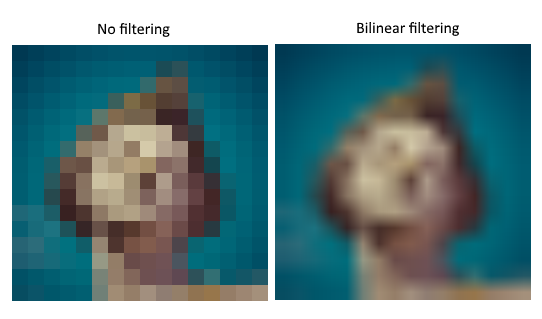
\includegraphics[width=\textwidth]{images/texture_filtering.png}
    \caption{Eine Textur als Lookup-Tabelle für Farbwerte. Ohne Interpolation (links) und mit bilinearer Interpolation (rechts). \cite{vulkan_tutorial:texture_filtering}}
    \label{fig:texture_filtering}
\end{figure}

Neben Buffern sind Texturen die zweite wichtige Datenstruktur für die \ac{GPU}. Eine Textur ist im Prinzip eine \textit{Lookup-Tabelle} \cite{wikipedia:lookup} mit 1-3 Dimensionen und der Möglichkeit zwischen den einzelnen \textit{Zellen} zu interpolieren (siehe Abbildung \ref{fig:texture_filtering}).

Dabei sind für das Erstellen einer \texttt{GPUTexture} besonders die Eigenschaften \texttt{dimension}, \texttt{textureSize}, \texttt{format} und \texttt{textureUsage} wichtig. Die \texttt{dimension} gibt die Anzahl der Dimensionen (\textit{1D}, \textit{2D} oder \textit{3D}) an. Die \texttt{textureSize} wiederum wie viele Texel (\textit{texture element} \cite{wikipedia:texel}) es in den jeweiligen Dimension gibt. Das heißt, ein \textit{1D}-Textur darf nur in einer Dimension mehr als ein Element haben (zum Beispiel (256, 1, 1)). Die einzelnen Eigenschaften der \texttt{textureSize} heißen dabei \texttt{width}, \texttt{height} und \texttt{depth}. Das \texttt{format} gibt an, was in jedem Texel gespeichert wird. Hier dürfte RGBA8 (also Rot, Grün, Blau und Alpha mit jeweils 8 Bit) wohl am bekanntesten sein. Jedoch gibt es sehr viele mehr, so sind aktuell 52 Texturformate in \textbf{WebGPU} verfügbar. \texttt{textureUsage} gibt an, wie die Texture benutzt werden soll, zum Beispiel zum Lesen oder zum Schreiben, als Kopierquelle oder Kopierziel, oder eine beliebige Kombination davon.

\begin{minipage}{\textwidth}
\begin{lstlisting}[language=JavaScript]
var texture = device.createTexture({
  size: {
  	width: 1024,
  	height: 1024,
  	depth: 1
  },
  mipLevelCount: 1,
  sampleCount: 1,
  dimension: '2d',
  format: 'rgba8unorm',
  usage: GPUTextureUsage.SAMPLED | GPUTextureUsage.COPY_DST 
});
\end{lstlisting}
\end{minipage}

Analog zu \texttt{writeBuffer} gibt es für Texturen auch eine \texttt{writeTexture}-Methode in der \texttt{GPUQueue}. Dies funktioniert allerdings nur, wenn die \texttt{GPUTexture} ein Kopierziel (\texttt{GPUTextureUsage.COPY\_DST}) ist. Um Daten in die \texttt{GPUTexture} zu kopieren, muss dafür unter anderem erst eine \texttt{GPUTextureCopyView} erstellt werden, die zum Beispiel den Offset der Kopieroperation festlegt, so dass auch zum Beispiel Daten nur in die Mitte der Textur geschrieben werden können. Hier ist anzumerken, dass die \texttt{writeTexture}-Methode zum Zeitpunkt des Verfassens dieses Abschnittes (28. Juni 2020) weder in Chromium, noch in Firefox Nightly implementiert ist.

\begin{minipage}{\textwidth}
\begin{lstlisting}[language=JavaScript]
var texture_data = new Uint32Array(1024 * 1024);
texture_data.fill(0x00FF00FF); // 0 red, 255 blue, 0 green, 255 alpha

var texture_copy_view = {
    texture: texture,
    mipLevel: 0,
    origin: {
        x: 0,
        y: 0,
        z: 0
    }
};
    
var data_layout = {
    offset: 0,
    bytesPerRow: 1024 * 4,
    rowsPerImage: 1024
};

var copy_size = {
    width: 1024,
    height: 1024,
    depth: 1
};
    
queue.writeTexture(texture_copy_view, texture_data, data_layout, copy_size);
\end{lstlisting}
\end{minipage}

Um die \texttt{GPUTexture} nun wirklich nutzen zu können, wird noch eine \texttt{GPUTextureView} benötigt, die beschreibt wie genau auf die Daten der \texttt{GPUTexture} zugegriffen wird. In den meisten Fällen reicht allerdings die Erzeugung einer \texttt{GPUTextureView} von der \texttt{GPUTexture} ohne Angabe zusätzlicher Optionen. Dann übernimmt die \texttt{GPUTextureView} die Eigenschaften der \texttt{GPUTexture}:

\begin{lstlisting}[language=JavaScript]
var texture_view = texture.createView();
\end{lstlisting}

\subsection{\texttt{GPUPipelineLayout}}
\label{sub:gpupipelinebase}
Die \texttt{GPUPipelineBase} beschreibt die Basis für \texttt{GPURenderPipeline} und \texttt{GPUComputePipeline}. Die Gemeinsamkeit aller Pipelines besteht darin, dass sie unter anderem ein Set von Eingaben bekommen und daraus wiederum ein Set aus Ausgaben erstellen. Die Eingaben und Ausgaben bestehen dabei grundlegend aus Buffern und Texturen. Dabei muss beim Erstellen einer Pipeline ihr \textit{Layout} festgelegt werden, d.h. was für Ressourcentypen benötigt werden und welche grundsätzlichen Eigenschaften diese Ressourcen haben. Die Eigenschaften umfassen zum Beispiel in welchem Shader (Vertex, Fragment oder Compute) die Ressourcen verfügbar sein sollen oder welche Dimension eine etwaige Textur hat.

Dabei ist zu beachten, dass hier nur die generelle Struktur der Ressourcen, aber nicht die Ressourcen an sich, festgelegt werden. Ein \texttt{GPUPipelineLayout} besteht dabei aus maximal 4 \texttt{GPUBindGroupLayout}s mit jeweils bis zu 16 \texttt{GPUBindGroupLayoutEntry}s. Diese Limitationen sind dabei die Mindestgrößen, die bei \textbf{WebGPU} garantiert werden. Je nach Hardware könnte hier auch mehr verfügbar sein. Generell ist es aber zu empfehlen, die Mindestgrößen zu verwenden, um eine Funktionalität auf möglichst vielen Geräten zu ermöglichen.

Als \textit{binding} wird die Verknüpfung einer Ressource mit dem jeweiligen Shader verstanden. Jedoch ist es nicht möglich ein einzelnes \textit{binding} zu ändern, sondern immer nur eine \textit{bind group}. Deshalb ist es sinnvoll die benötigten \textit{bindings} so in die \textit{bind groups} aufzuteilen, dass ein unnötiges Aktualisieren von \textit{bindings}, die nicht aktualisiert werden müssen, vermieden wird. Als Beispiel könnte man hier einen Vertex-Shader sehen, der für jedes Modell die gleichen \textit{View}- und \textit{Projection}-Matrizen verwenden kann (da sich die Kamera nicht innerhalb eines \textit{frames} verändert, aber jeweils die \textit{Model}-Matrix aktualisieren muss (siehe Abschnitt \ref{sub:geometry_processing}). Hier könnte man dann zwei \textit{bind groups} mit jeweils einem \textit{binding} zu einem Buffer erstellen. Wobei ein Buffer hier die \textit{View}- und \textit{Projection}-Matrizen beinhaltet, so dass dieses \textit{binding} nur einmal gesetzt werden muss. Das \textit{binding} zum anderen Buffer, welcher die jeweilige \textit{Model}-Matrix beinhaltet, muss dabei für jedes Modell aktualisiert werden.

\begin{minipage}{\textwidth}
\begin{lstlisting}[language=JavaScript]
// bgle = BindGroupLayoutEntry
// bgl = BindGroupLayout

var bgle_view_proj = {
    binding: 0,
    visibility: GPUShaderStage.VERTEX,
    type: 'uniform-buffer',
    hasDynamicOffset: false
};

var bgl_common = device.createBindGroupLayout({
    entries: [
        bgle_view_proj
    ]
});

var bgle_model = {
    binding: 0,
    visibility: GPUShaderStage.VERTEX,
    type: 'uniform-buffer',
    hasDynamicOffset: true
};

var bgl_update = device.createBindGroupLayout({
    entries: [
        bgle_model
    ]
});

var pipeline_layout = device.createPipelineLayout({
    bindGroupLayouts: [
        bgl_common,
        bgl_update
    ]
});
\end{lstlisting}
\end{minipage}

Das Attribut \texttt{binding} eines \texttt{BindGroupLayoutEntry} gibt hierbei einen Index an, der im Shader benutzt wird, um die Ressource innerhalb der \textit{bind group} zu identifizieren. Im Shader wird die jeweilige \textit{bind group} dann mit \texttt{set} identifiziert, was sich auf den Index des jeweiligen \texttt{GPUBindGroupLayout} in \texttt{GPUPipelineLayout.bindGroupLayouts} bezieht (siehe Listing \ref{lst:set_binding}).

\begin{lstlisting}[language=GLSL, label={lst:set_binding}, caption={Deklaration der Buffer im Shader. \texttt{set} identifiziert hierbei die \textit{bind group}, und \texttt{binding} die Ressource innerhalb der \textit{bind group}.}]
layout(set = 0, binding = 0) uniform Common {
	mat4 view;
	mat4 proj;
} common;

layout(set = 1, binding = 0) uniform Update {
	mat4 model;
} update;

...
\end{lstlisting}

\subsection{\texttt{GPURenderPipeline}}
\begin{table}[htb]
\begin{center}
\begin{tabular}{ |l|l|p{6cm}| }
    \hline
    \textbf{\#} & \textbf{WebGPU-Objekt} & \textbf{Beschreibung} \\
    \hline
    \rowcolor{lightorange}
    \texttt{1} & \texttt{GPUVertexStateDescriptor} & Beschreibt das Format der Indexdaten (\texttt{Uint16} oder \texttt{Uint32}) und das Layout der einzelnen Vertexbuffer  \\
    \hline
    \rowcolor{lightgreen}
    \texttt{2} & \texttt{GPUShaderModule} & Vertex-Shader \\
    \hline
    \rowcolor{lightorange}
    \texttt{3} & \texttt{GPUPrimitiveTopology} & Beschreibt wie die Liste der Vertices aufgefasst werden soll (Punkte, Linien oder Dreiecke) \\
    \hline
    \rowcolor{lightorange}
    \texttt{4} & \texttt{GPURasterizationStateDescriptor} & Beschreibt wie die Vorderseite eines Dreiecks ermittelt werden soll und welche Seiten verworfen werden sollen \\
    \hline
    \rowcolor{lightgreen}
    \texttt{5} & \texttt{GPUShaderModule} & Pixel- bzw. Fragment-Shader \\
    \hline
    \rowcolor{lightorange}
    \texttt{6} & \texttt{GPUDepthStencilStateDescriptor} & Beschreibt die Tests und Operationen für den \textit{stencil} (Bitmaske) und \textit{depth buffer} \\
    \hline
    \rowcolor{lightorange}
    \texttt{7} & \texttt{GPUColorStateDescriptor} & Beschreibt wie die Resultate von Abschnitt 5 in den \textit{color buffer} gemischt werden sollen \\
    \hline
\end{tabular}
\end{center}
Legende: \colorbox{lightorange}{nur konfigurierbar} \colorbox{lightgreen}{frei programmierbar}
\caption{Beschreibung der Abschnitte von \texttt{GPURenderPipeline}}
\label{tab:render_pipeline_stages}
\end{table}

Die \texttt{GPURenderPipeline} bildet die im Abschnitt \ref{sec:render_pipeline} beschriebene Rendering-Pipeline im \textbf{WebGPU}-Kontext. Dabei produziert sie aus den Eingaben mithilfe von einer Reihe von jeweils festen oder frei programmierbaren Abschnitten Ausgaben. Die Eingaben bestehen dabei, zusätzlich zu den \textit{bindings} jeder Pipeline, aus Vertex bzw. Indexdaten und \textit{color} und \textit{depth buffers}, die zum Start entweder geleert oder übernommen werden können. Die Ausgaben bestehen dabei aus den (eventuell) veränderten \textit{color} und \textit{depth buffers} und optional werden auch ein Teil der \textit{bindings} (zum Beispiel \textit{storage buffer}s oder \textit{writeonly-storage-texture}s) verändert.

Die Rendering-Pipeline ist dabei in 6 nur konfigurierbare und 2 gänzlich frei programmierbare Abschnitte aufgeteilt (siehe Tabelle \ref{tab:render_pipeline_stages}).

Mit diesen Informationen und dem \texttt{GPUPipelineLayout} aus Abschnitt \ref{sub:gpupipelinebase} lässt sich nun eine \texttt{GPURenderPipeline} erstellen (siehe Listing \ref{lst:renderpipeline}).

\begin{lstlisting}[language=JavaScript, label={lst:renderpipeline}, caption={Erstellen einer \quotize{Standard}-\texttt{GPURenderPipeline}}]
var render_pipeline = device.createRenderPipeline({
    layout: pipeline_layout,
    vertexState: {
        indexFormat: 'uint16',
        vertexBuffers: [
            {
                arrayStride: 24, // 24 bytes per vertex
                stepMode: 'vertex',
                attributes: [
                    { // pos attribute
                        format: 'float3',
                        offset: 0,
                        shaderLocation: 0
                    },
                    { // color attribute
                        format: 'float3',
                        offset: 12, // offset in bytes
                        shaderLocation: 1
                    }
                ]
            }
        ]
    },
    vertexStage: {
        module: device.createShaderModule({
            code: VertexShaderCode
        }),
        entryPoint: 'main'
    },
    primitiveTopology: 'triangle-list',
    rasterizationState: {
        frontFace = 'ccw', // counter clock wise
        cullMode = 'none', // don't cull faces
    },
    fragmentStage: {
        module: device.createShaderModule({
            code: FragmentShaderCode
        }),
        entryPoint: 'main'
    },
    depthStencilState: {
        format: 'depth32float',
        depthWriteEnabled: true,
        depthCompare: 'greater'
    }
    colorStates: [
        {
            format: 'rgba8srgb',
            alphaBlend: { 
                srcFactor: 'one', 
                dstFactor: 'zero', 
                operation: 'add'
            },
            colorBlend: { 
                srcFactor: 'one', 
                dstFactor: 'zero', 
                operation: 'add'
            },
            writeMask: GPUColorWrite.ALL
        }
    ]
});
\end{lstlisting}

\subsection{\texttt{GPUBindGroup}}
Um die Ressourcen nun in der \texttt{GPURenderPipeline} nutzen zu können, müssen diese in \texttt{GPUBindGroup}s zusammengefasst werden. Dabei beschreibt eine \texttt{GPUBindGroup} die tatsächliche Verknüpfung von Ressourcen auf Grundlage eines \texttt{GPUBindGroupLayout}. Analog dazu beschreibt ein \texttt{GPUBindGroupLayoutEntry} die grundlegende Struktur der zu verknüpfenden Ressource und \texttt{GPUBindGroupEntry} beschreibt die tatsächliche Verknüpfung. Dazu müssen wir aber erst die jeweiligen Ressourcen erstellen. In unserem Fall sind das 2 Buffer vom Typ \textit{uniform}, d.h die Daten in den Buffern sind für jeden Shader-Aufruf gleich und unterscheiden sich nicht zwischen den einzelnen \textit{vertices} (oder \textit{fragments}). In einem Buffer werden dabei die \textit{View}- und \textit{Projection}-Matrizen gespeichert und in dem anderen die \textit{Model}-Matrix (siehe Listing \ref{lst:uniform_buffers}). 

\begin{minipage}{\textwidth}
\begin{lstlisting}[language=JavaScript, label={lst:uniform_buffers}, caption={Erstellen der Uniform-Buffer für einerseits \textit{common data} (\textit{View}- / \textit{Projection}-Matrix) und anderseits \textit{dynamic data} (\textit{Model}-Matrix).}]
const fovy_rad = 60.0 * PI / 180.0;
const f = 1.0 / Math.tan(fovy_rad * 0.5);
const aspect = 800.0 / 600.0;
var common_data = new Float32Array([
    // view matrix
    1.0, 0.0, 0.0, 0.0,
    0.0, 1.0, 0.0, 0.0,
    0.0, 0.0, 1.0, 0.0,
    0.0, 0.0, 0.0, 1.0,
    // proj matrix
    f / aspect, 0.0, 0.0, 0.0,
    0.0, f, 0.0, 0.0,
    0.0, 0.0, 0.0, 0.1,
    0.0, 0.0, -1.0, 0.0
]);

var common_buffer = device.createBuffer({
    size: common_data.byteLength,
    usage: GPUBufferUsage.UNIFORM
});

queue.writeBuffer(common_buffer, 0, common_data);

var model_data = new Float32Array([
    // model matrix (moved 2 units in Z direction)
    1.0, 0.0, 0.0, 0.0,
    0.0, 1.0, 0.0, 0.0,
    0.0, 0.0, 1.0, 2.0,
    0.0, 0.0, 0.0, 1.0
]);

var dynamic_buffer = device.createBuffer({
    size: model_data.byteLength,
    usage: GPUBufferUsage.UNIFORM
});

queue.writeBuffer(dynamic_buffer, 0, model_data);
\end{lstlisting}
\end{minipage}

Da wir in Abschnitt \ref{sub:gpupipelinebase} 2 \texttt{GPUBindGroupLayout}s mit jeweils 1 \texttt{GPUBindGroupLayoutEntry} erstellt haben, müssen wir nun passenden \texttt{GPUBindGroup}s und \texttt{GPUBindGroupEntry}s erstellen (siehe Listing \ref{lst:bind_groups}).

\begin{minipage}{\textwidth}
\begin{lstlisting}[language=JavaScript, label={lst:bind_groups}, caption={Erstellen der \texttt{GPUBindGroup}s für \textit{common} und \textit{dynamic data}.}]
var bind_group_common = device.createBindGroup({
    layout: bgl_common,
    entries: [
        {
            binding: 0,
            resource: {
                buffer: common_buffer,
                offset: 0,
                size: common_data.byteLength
            }
        }
    ]
});

var bind_group_dynamic = device.createBindGroup({
    layout: bgl_dynamic,
    entries: [
        {
            binding: 0,
            resource: {
                buffer: dynamic_buffer,
                offset: 0,
                size: model_data.byteLength
            }
        }
    ]
});
\end{lstlisting}
\end{minipage}

\subsection{\texttt{GPUSwapChain}}
Um nun unsere Modelle zu rendern zu können brauchen wir noch eine Textur, in die wir das fertige Bild schreiben können, den \textit{color buffer}. Diese Textur bekommen wir von der \textit{swap chain} \cite{wikipedia:swap_chain} zugeteilt. Dazu müssen wir aber erst ein \texttt{GPUSwapChain}-Objekt erstellen. Die \texttt{GPUSwapChain} können wir von einem \texttt{HTMLCanvasElement} bekommen (siehe Listing \ref{lst:canvas_swap_chain}).

\begin{minipage}{\textwidth}
\begin{lstlisting}[language=JavaScript, label={lst:canvas_swap_chain}, caption={Erstellen einer \texttt{GPUSwapChain} von einem \texttt{HTMLCanvasElement}}]
var canvas = document.getElementById('canvas');
var canvas_context = canvas.getContext('gpupresent');
var swap_chain = canvas_context.configureSwapChain({
    device: device,
    format: 'rgba8srgb',
    usage: GPUTextureUsage.OUTPUT_ATTACHMENT
});
\end{lstlisting}
\end{minipage}

\section{Rendering}
Die Schritte in diesem Abschnitt müssen für jeden \textit{frame} betätigt werden. Es ist zwar möglich, dies nur einmal zu machen, um zum Beispiel ein statisches Bild zu generieren. Für eine interaktive Applikation oder zum Beispiel einen Video-Player sollte die Wiederholrate an das Ausgabegerät angepasst werden, was meist um die 60 Hertz bzw. Bilder die Sekunde sind.

\subsection{\texttt{GPUCommandEncoder}}
Ein \texttt{GPUCommandEncoder} nimmt Befehle für die \ac{GPU} auf. Um zum Beispiel den Inhalt eines \texttt{GPUBuffer} in einen anderen zu kopieren, kann die Methode \texttt{copyBufferToBuffer} benutzt werden. Hierbei ist aber wichtig zu beachten, dass die Befehle nicht direkt ausgeführt werden, sondern nur aufgenommen werden. Um die Befehle dann tatsächlich auf der \ac{GPU} ausführen zu lassen, muss ein \texttt{GPUCommandBuffer} erstellt werden (siehe Abschnitt \ref{sub:command_buffer}). Die Erstellung eines \texttt{GPUCommandEncoder} ist dabei trivial (siehe Listing \ref{lst:command_encoder}).

\begin{lstlisting}[language=JavaScript, label={lst:command_encoder}, caption={Erstellen eines \texttt{GPUCommandEncoder}}]
var command_enc = device.createCommandEncoder();
\end{lstlisting}

\subsection{\texttt{GPURenderPassEncoder}}
Um nun die \textit{Render}-Befehle aufzunehmen, muss erst ein \texttt{GPURenderPassEncoder} vom \texttt{GPUCommandEncoder erstellt werden}. Der \texttt{GPURenderPassEncoder} benötigt dabei zur Erstellung den \textit{color} und \textit{depth buffer}. Den \textit{color buffer} bzw. die \textit{color texture} erhalten wir dabei von der \texttt{GPUSwapChain} und den \textit{depth buffer} bzw. die \textit{depth texture} erstellen wir jedes Mal neu (siehe Listing \ref{lst:render_pass}).

\begin{minipage}{\textwidth}
\begin{lstlisting}[language=JavaScript, label={lst:render_pass}, caption={Erstellen eines \texttt{GPURenderPassEncoder} vom \texttt{GPUCommandEncoder}. Die benötigte \textit{color texture} bekommen wir von der \texttt{GPUSwapChain} und die benötigte \textit{depth texture} erstellen wir jedes Mal neu.}]
var color_texture = swap_chain.getCurrentTexture();
var depth_texture = device.createTexture({
    size: {
        width: canvas.width,
        height: canvas.height,
        depth: 1
    },
    mipLevelCount: 1,
    sampleCount: 1,
    dimension: '2d',
    format: 'depth32float',
    usage: GPUTextureUsage.OUTPUT_ATTACHMENT
});

var render_pass = command_enc.beginRenderPass({
    colorAttachments: [
        {
            attachment: color_texture.createView(),
            loadValue: {r: 0.3, g: 0.0, b: 0.2, a: 1.0}, // clear to dark purple
            storeOp: 'store'
        }
    ],
    depthStencilAttachment: {
        attachment: depth_texture.createView(),
        depthLoadValue: 0.0,
        depthStoreOp: 'store',
        depthReadOnly: false,
        stencilLoadValue: 0,
        stencilStoreOp: 'store',
        stencilReadOnly: true
    },
});
\end{lstlisting}
\end{minipage}

Dem nun erstellten \texttt{GPURenderPassEncoder} können wir nun die \texttt{GPURenderPipeline}, die Vertex- und Index-Buffer, sowie die zwei \textit{GPUBindGroup}s zuweisen und dann einen Befehl zum \textit{rendern} des Modells aufnehmen (siehe Listing \ref{lst:render}). Auch die Befehle zum Setzen der Ressourcen werden hier nur aufgenommen (in dem \texttt{GPUCommandEncoder} mit dem der \texttt{GPURenderPassEncoder} erstellt wurde) und erst später ausgeführt.

\begin{lstlisting}[language=JavaScript, label={lst:render}, caption={Erstellen einer \texttt{GPUSwapChain} von einem \texttt{HTMLCanvasElement}}]
render_pass.setPipeline(render_pipeline);
render_pass.setVertexBuffer(0, vertex_buffer);
render_pass.setIndexBuffer(index_buffer);
render_pass.setBindGroup(0, bind_group_common);
render_pass.setBindGroup(1, bind_group_dynamic);
render_pass.drawIndexed(index_data.length);
render_pass.endPass();
\end{lstlisting}

\subsection{\texttt{GPUCommandBuffer}}
\label{sub:command_buffer}
Haben wir nun alle benötigten Befehle aufgenommen können wir ein \texttt{GPUCommandBuffer} vom \texttt{GPUCommandEncoder} generieren und die Befehle mithilfe der \texttt{GPUQueue} zur \ac{GPU} schicken (siehe Listing \ref{lst:submit}).

\begin{lstlisting}[language=JavaScript, label={lst:submit}, caption={Generieren eines \texttt{GPUCommandBuffer} und Abschicken der Befehle an die GPU.}]
var command_buffer = command_enc.finish();
queue.submit([command_buffer]);
\end{lstlisting}

\section{Resultat}
\begin{figure}
    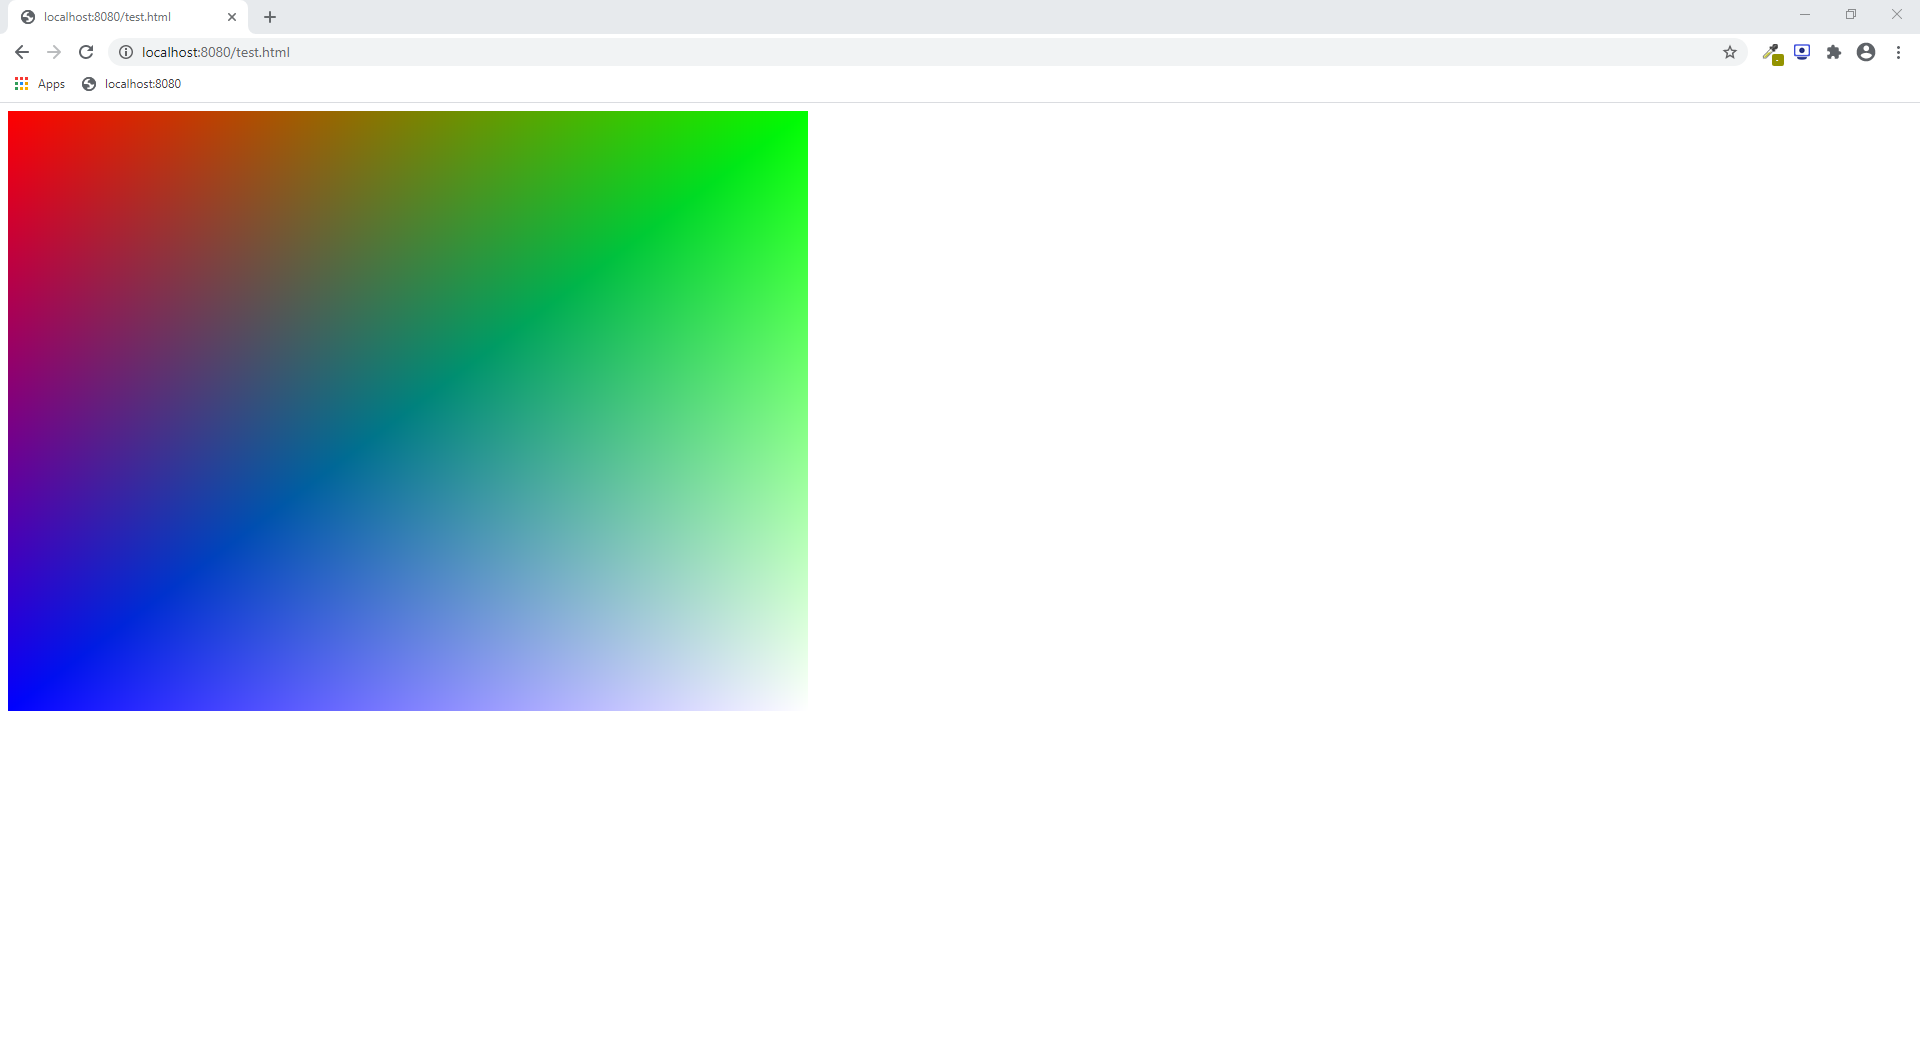
\includegraphics[width=\textwidth]{images/simple_result.png}
    \caption{Resultat des Minimalbeispiels in Google Chrome Canary.}
    \label{fig:simple_result}
\end{figure}
Wie in Abbildung \ref{fig:simple_result} zu sehen, erhalten wir nun ein farbiges Bild in unserem HTML-Canvas. Dabei haben wir nur die Eckpunkte und ihre jeweiligen Farben spezifiziert und die \ac{GPU} hat die Farben für die inneren Pixel aus den Vertexdaten interpoliert.

Dabei ist zu beachten, dass dieses Minimalbeispiel nicht darauf ausgelegt ist ein beachtliches Resultat zu erzeugen, sondern es soll mehr einen Querschnitt durch die \textbf{WebGPU} aufzeigen und veranschaulichen, was dazu nötig ist, eine sehr simple Applikation zu erstellen. Da der größte Teil des Aufwands hierbei in der Initialisierung steckt, kann die Applikation nun mit relativ wenig Aufwand erweitert werden. Dazu müssen primär nur noch die einzelnen Ressourcen (Vertex-, Index- und Uniform-Buffer) und die Shader erweitert werden. An der Grundstruktur muss nicht mehr viel angepasst werden.
%---
\chapter{Die spider-Engine}
\label{cha:spider}
\textit{Für das in diesem Kapitel beschriebene Projekt wurde Windows 10 mit Ubuntu 19.10 per \ac{WSL} \cite{microsoft:wsl} verwendet. Dabei wurden die Quellcodedateien in Windows erstellt und bearbeitet, aber in Ubuntu benutzt (kompilieren, linken usw.). Deshalb beziehen sich im Folgenden alle Angaben zur Installation oder Benutzung von Werkzeugen auf die jeweilige Linux-Version.}

\section{spider}
\label{sec:spider}
\textit{In diesem Abschnitt wird mit \quotize{der Benutzer}, ein Benutzer der \textbf{spider}-Engine verstanden, also eine Person, die mithilfe der Engine eine eigene Applikation entwickelt. \quotize{Der Benutzer} sollte hier als neutrale Form, die die weibliche, sowie die männliche Form beinhaltet, verstanden werden.}
\subsection{Überblick}
\label{sub:overview}
Mit der parallel zu dieser Arbeit entstandenen \textbf{spider}-Engine, lässt sich mit geringem Aufwand eine Webapplikation zur Darstellung von 3D-Szenen in C/C++ erstellen.
Das Grundgerüst dafür ist sehr minimal (siehe Listing \ref{lst:spider_base}).

\begin{minipage}{\textwidth}
\begin{lstlisting}[language=C, label={lst:spider_base}, caption={Grundgerüst einer Applikation mit der \textbf{spider}-Engine}]
#include "spider/spider.h"

// Create the initial state of your scene
void initApplication();
// Update your scene each frame
bool update(float delta_time_s);

int main() {
	const uint32_t surface_width = 1280;
	const uint32_t surface_height = 720;

	// Initialize the spider engine
	spInit(&(SPInit){
		.surface_size = {
			.width = surface_width,
			.height = surface_height
		},
		.update_func = update,
		.camera = {
			.pos = {0.0f, 2.0f, 5.0f},
			.look_at = {0.0f, 0.0f, 0.0f},
			.mode = SPCameraMode_LookAt,
			.fovy = glm_rad(60.0f),
			.aspect = (float)surface_width / (float) surface_height,
			.near = 0.1f,
		},
	});	
	
	initApplication();
	spStart();
	
	return 0;
}

void initApplication() {
	// Here you can create lights (only spotlights for now),
	// create custom meshes and materials 
	// or load them from glTF files (recommended)
}

bool update(float delta_time_s) {
	// Here you can update your created lights, objects and the main camera
	
	// Return false, if you want to quit the application
	return true;
}
\end{lstlisting}
\end{minipage}

Die \textbf{spider}-Engine ist darauf ausgelegt, mit möglichst wenig Code auf Seiten des Benutzers eine 3D-Applikation zu erstellen. So lässt sich in rund 150 Zeilen Code eine interaktive 3D-Szene mit einem UserInterface (dank integriertem Dear ImGui \cite{dear_imgui}) erstellen (siehe Abbildung \ref{fig:spider_example_sponza} und Anhang \ref{appendix:a}). Trotzdem ist die Funktionalität der \textbf{spider}-Engine sehr beschränkt, wenn man etwas anderes als das Darstellen von 3D-Modellen und eines einfachen UserInterfaces will. Jedoch ist der Verfasser überzeugt, dass es für einfache Prototypen ausreichend ist.

\begin{figure}
    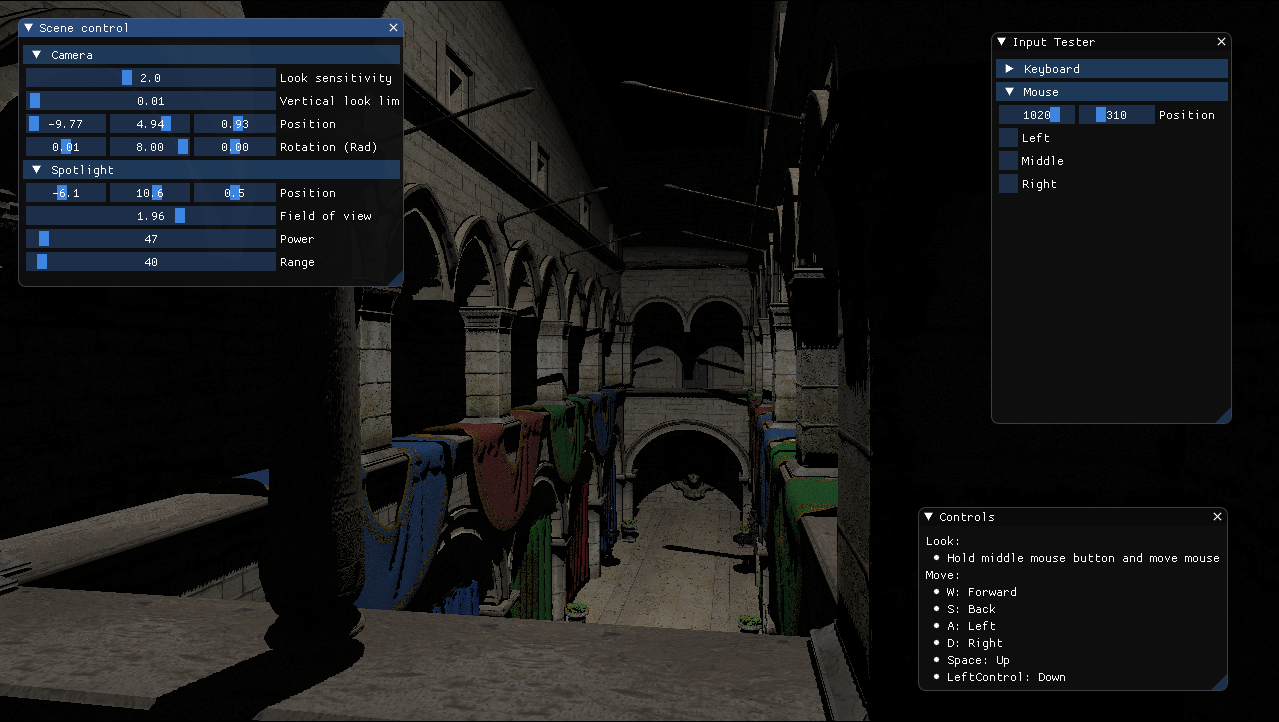
\includegraphics[width=\textwidth]{images/state_of_work_20200608.png}
    \caption{Interaktive 3D-Szene mit UserInterface. Bildschirmaufnahme durch Verfasser.}
    \label{fig:spider_example_sponza}
\end{figure}

\subsection{Codestyle}
\label{sub:codestyle}
\textit{Für das Projekt wurde der C Standard C99 und der von \textbf{Emscripten} verwendete Compiler clang benutzt. Folgende Punkte sollten in allen größeren C-Compilern, die C99 unterstützen, problemlos funktionieren, wurden dort aber nicht getestet.}

Um einen einheitlichen Codestyle zu erhalten, hat der Verfasser sich auf folgende Punkte festgelegt:

\subsubsection{\textit{stdint.h} und \textit{stdbool.h}}
Im Projekt wurden die seit C99 verfügbaren Headerdateien \texttt{stdint.h} und \texttt{stdbool.h} benutzt, um einerseits mehr Kontrolle über den Speicherbedarf der jeweiligen Komponenten zu erlangen und anderseits mehr Kontext zu geben. So ist zum Beispiel bei einer Variable des Typen \texttt{uint8\_t} schnell klar, dass der Verfasser für die Benutzung der Variable nur einen relativ kleinen Bereich an positiven Ganzzahlen beabsichtigt hat. Auch der Typ \texttt{bool} ist im Vergleich zu einem \texttt{int} eindeutig im Bezug auf die Absicht des Verfassers. Interessanterweise wurde beim gesamten Projekt (außer bei der Kommunikation mit den verwendeten Bibliotheken) nur Ganzzahldatentypen ohne Vorzeichen benutzt (\texttt{uint8\_t}, \texttt{uint16\_t}, \texttt{uint32\_t} und \texttt{uint64\_t}).

\subsubsection{Prefixe}
Da es in C keine Namensbereiche, wie zum Beispiel in C++, gibt, werden alle Strukturen, Enums, Funktionen, Preprozessordirektiven und globale Variablen mit einem Prefix versehen (siehe Tabelle \ref{tab:prefixes}). Die Unterscheidung zwischen \textit{öffentlich} und \textit{privat} ist hierbei keine Unterscheidung auf Compilerlevel, sondern nur für den Benutzer, damit dieser erkennen kann, welche Funktionen und Strukturen benutzt werden sollten und welche nur intern genutzt werden.

\begin{table}
\begin{center}
\begin{tabular}{ |l|l|l| }
\hline
\textbf{Typ} & \textbf{Prefix} & \textbf{Beispiel} \\
\hline
\multicolumn{3}{|c|}{\quotize{öffentlich}} \\
\hline
Struktur & \texttt{SP} & \texttt{SPMesh} \\
\hline
Enum & \texttt{SP} & \texttt{SPKey} \\
\hline
Funktion & \texttt{sp} & \texttt{spInit} \\
\hline
Preprozessordirektive & \texttt{SP\_} & \texttt{SP\_INVALID\_ID} \\
\hline
globale Variable & \texttt{sp\_} & \textit{kein Beispiel} \\
\hline
\multicolumn{3}{|c|}{\quotize{privat}} \\
\hline
Struktur & \texttt{\_SP} & \texttt{\_SPRenderPipeline} \\
\hline
Enum & \texttt{\_SP} & \textit{kein Beispiel} \\
\hline
Funktion & \texttt{\_sp} & \texttt{\_spSetupPools} \\
\hline
Preprozessordirektive & \texttt{\_SP\_} & \texttt{\_SP\_MATERIAL\_POOL\_DEFAULT} \\
\hline
globale Variable & \texttt{\_sp\_} & \texttt{\_sp\_state} \\
\hline
\end{tabular}
\end{center}
\caption{In der \textbf{spider}-Engine verwendete Prefixe}
\label{tab:prefixes}
\end{table}

\subsubsection{Definition von Strukturen}
Strukturen werden im Projekt wie in Listing \ref{lst:structs} definiert.

\begin{minipage}{\textwidth}
\begin{lstlisting}[language=C, label={lst:structs}, caption={Definition von Strukturen}]
typedef struct MyStructure {
	uint32_t x;
	struct {
		float width;
		float height;
	} size;
} MyStructure;
\end{lstlisting}
\end{minipage}

Dies hat den Vorteil, dass die so definierten Strukturen nicht immer ein vorhergehendes \texttt{struct} bei der Verwendung im Code benötigen. Zusätzlich wird direkt nach dem \texttt{struct} auch der Name der Struktur benötigt, damit diese weiterhin vorwärts deklariert werden kann \cite[vgl.][]{weissflog:structs}. 

Semantisch zusammengehörige Attribute innerhalb einer Struktur werden entweder in eine extra Struktur ausgelagert, oder als anonyme Struktur (siehe \texttt{size} im Beispiel) innerhalb der Struktur definiert. Dadurch kann über \texttt{my\_structure.size.width} auf das Attribut zugegriffen werden.

\subsubsection{\textit{Desc}-Argument}
In vielen Programmiersprachen ist es möglich, beim Aufrufen einer Funktion nur einen Teil der Argumente anzugeben, während die restlichen Argumente mit Standardwerten initialisiert werden. C unterstützt zwar keine Standardargumente, dafür aber ab C99 \textit{Bestimmte Initialisierer (engl. designated initializers)}, was bedeutet, dass man die Felder von Strukturen (und Arrays) mit ihrem jeweiligen Namen (oder Index) in beliebiger Reihenfolge innerhalb einer Initialisierungsanweisung angeben kann. Wenn mindestens ein Feld initialisiert wird, werden alle nicht initialisierten Felder mit \textbf{0} initialisiert. (Zur Verdeutlichung siehe Listing \ref{lst:designated_initializers}). 

\begin{minipage}{\textwidth}
\begin{lstlisting}[language=C, label={lst:designated_initializers}, caption={Beispiele zu bestimmten Initialisierern (Unter Verwendung der in Listing \ref{lst:structs} definierten Struktur \textit{MyStructure})}]
// No guarantee on initialization values
MyStructure my_structure;

// Initialization in field order 
// -> (x = 5, size.width = 3.0f, size.height = 4.0f)
MyStructure my_structure_order = {5, {3.0f, 4.0f}};
MyStructure my_structure_order2 = {5, 3.0f, 4.0f};

// Initialization in field order, rest is zero initialized
// -> (x = 5, size.width = 0.0f, size.height = 0.0f)
MyStructure my_structure_order_zero = {5};

// Initialization with field names
// -> (x = 5, size.width = 3.0f, size.height = 4.0f)
MyStructure my_structure_named = {.size.width = 3.0f, .x = 5, .size.height = 4.0f};
MyStructure my_structure_named2 = {.size = {.width = 3.0f, .height = 4.0f }, .x = 5};

// Initialization with field names, rest is zero initialized
// -> (x = 0, size.width = 3.0f, size.height = 0.0f)
MyStructure my_structure_named_zero = {.size.width = 3.0f};
MyStructure my_structure_named_zero2 = {.size = {.width = 3.0f}};

// Initialization of array fields
// -> (0, 3, 0, 0, 1)
uint32_t array[5] = {
	[1] = 3,
	[4] = 1
};
\end{lstlisting}
\end{minipage}

Im Projekt wird das bei Funktionen mit einer nicht trivialen Argumentliste verwendet. Dabei wird für die jeweilige Funktion eine Struktur mit dem Postfix \texttt{Desc} (für engl. \textit{descriptor}, analog zu den \textbf{WebGPU}-\textit{Descriptor}-Strukturen) definiert. Diese enthält alle benötigten Argumente (mit möglichst sinnvollem Standardwert \textbf{0}). Da es außerdem in C99 möglich ist, einen Zeiger auf ein temporäres Objekt zu erzeugen, hat die jeweilige Funktion nun als einziges Argument einen Zeiger auf ein konstantes Objekt der \texttt{Desc}-Struktur: \texttt{void myFunction(const MyFunctionDesc* desc);}. Nun kann die \texttt{Desc}-Struktur entweder vor dem Aufrufen der Funktion erschaffen und befüllt werden, oder direkt beim Funktionsaufruf initialisiert werden (siehe Listing \ref{lst:function_desc}).

\begin{minipage}{\textwidth}
\begin{lstlisting}[language=C, label={lst:function_desc}, caption={Verwendung einer \textit{Desc}-Struktur zum Übergeben von Argumenten an eine Funktion}]
typedef struct MyFunctionDesc {
	uint32_t values[5];
	const char* name;
} MyFunctionDesc;

void myFunction(const MyFunctionDesc* desc);

MyFunctionDesc my_desc;
my_desc.values[2] = 5;
my_desc.name = "Abc";
myFunction(&my_desc);

myFunction(&(MyFunctionDesc){
	.values = {
		[2] = 5,
	},
	.name = "Abc",
});
\end{lstlisting}
\end{minipage}

\subsubsection{\textit{handles} \cite[Vgl.][]{weissflog:handles}}
\label{subsub:handles}

Die \textbf{spider}-Engine hat das Grundprinzip, dass der Benutzer sich weder um die (De-)Allokation von Speicher, noch über die Referenzierungen zwischen Objekten, kümmern muss und somit den vollen Fokus auf die Erstellung der jeweiligen Applikation richten kann. Dabei soll auch die Speicherverwaltung von erschaffenen Objekten (zum Beispiel ein \texttt{SPMesh}) einzig der \textbf{spider}-Engine überlassen werden. Dabei soll die Engine auch die Möglichkeit haben, die jeweiligen Objekte intern zu verschieben und zu sortieren (bisher nicht benutzt) um den internen Zugriff zu optimieren. Daher kann die Engine nicht direkt einen Zeiger auf ein erschaffenes Objekt liefern, da dieser bei einer Änderung der internen Struktur ungültig wird.

Dafür gibt es für jede \textit{öffentliche} Struktur eine \textit{handle}-Struktur mit Postfix \textit{ID} (zum Beispiel für \texttt{SPMesh} -> \texttt{SPMeshID}) welche eine interne ID (\textit{uint32\_t id}) beinhaltet. Bisher wird die interne ID des \textit{handle} einfach direkt als Index in das interne Array zur Verwaltung der jeweiligen Objekte benutzt, jedoch könnte man hier noch ähnlich zu \cite{weissflog:handles} die unbenutzten Bits (bei zum Beispiel maximal $2^{16} = 65536$ gleichzeitig existierenden Objekten bleiben hier 16 von 32 Bits übrig) zur Versionierung des \textit{handle} verwenden. Um das referenzierte Objekt dann im Anwendungscode zu benutzen kann ein temporärer Zeiger erzeugt werden (siehe Listing \ref{lst:handle}). Dieser Zeiger sollte vom Benutzter nicht gespeichert werden und nur erzeugt werden, wenn das referenzierte Objekt wirklich verwendet (Attribute lesen oder schreiben) wird. Es gibt keine Garantie, dass der Zeiger im nächsten Update noch auf das gleiche Objekt zeigt, oder überhaupt gültig ist.

\begin{minipage}{\textwidth}
\begin{lstlisting}[language=C, label={lst:handle}, caption={Verwendung von \textit{handles}}]
typedef struct SPObject {
	float size;
} SPObject;

typedef struct SPObjectID {
	uint32_t id;
} SPObjectID;

// Store the object handle
SPObjectID object_id;

void init() {
	// Create object and store the handle
	object_id = spCreateObject();
}

void update() {
	// Later use the referenced object
	SPObject* object = spGetObject(object_id);
	// If handle is not valid, spGetObject returns a NULL pointer
	if(object) {
		object->size *= 2.0f;
	}
}
\end{lstlisting}
\end{minipage}

\section{emscripten \cite{emscripten}}
Augenscheinlich wurde das Projekt, das diese Arbeit begleitet hat, in C geschrieben. Da die entstandene Applikation jedoch später in einem Webbrowser laufen und dort die \textbf{WebGPU}-\ac{API} benutzen soll, muss der C-Quellcode in ein Format umgewandelt werden, welches ein Webbrowser verstehen kann. Dazu wird das Werkzeug \textbf{Emscripten} verwendet. Mit \textbf{Emscripten} lässt sich (unter anderem) C-Quellcode mit Hilfe von LLVM \cite{llvm} zu JavaScript und WebAssembly \cite{wasm} kompilieren.

\subsection{Funktionsweise}
Um \textbf{Emscripten} benutzen zu können, muss als erstes das Emscripten SDK (emsdk) heruntergeladen und installiert werden \cite{emsdk}. Am einfachsten ist es hierbei, das SDK im gleichen Ordner zu platzieren, wie das Projekt, das es benutzen soll:
\dirtree{% 
.1 path\textbackslash.
	.2 to\textbackslash.
		.3 emsdk\textbackslash.
		.3 my\_project\textbackslash.
			.4 test.c.
}
Zum Beginn einer Terminal-Sitzung müssen noch die Umgebungsvariablen für \textbf{Emscripten} gesetzt werden (dies macht man am besten im \textit{path\textbackslash to\textbackslash emsdk\textbackslash}-Ordner):

\texttt{source ./emsdk\_env.sh}

Im Projektordner (\textit{path\textbackslash to\textbackslash my\_project\textbackslash}) kann nun die C-Quellcodedatei kompiliert werden:

\texttt{./emcc test.c -WASM=1 -o test.html}

Dadurch entstehen folgende Dateien:
\begin{itemize}
\item \texttt{test.html}: Eintrittspunkt für die Web-Applikation
\item \texttt{test.wasm}: Kompilierter C-Code in WebAssembly
\item \texttt{test.js}:   JavaScript-Code zur Verknüfung von HTML, JavaScript und WebAssembly
\end{itemize}

\section{Besonderheiten bei der Entwicklung einer GPU Applikation}
Dadurch, dass viele Befehle nicht auf der \ac{CPU}, sondern auf der \ac{GPU} ablaufen, sind traditionelle \textit{Debugger}, wie \textit{gdb}, nur begrenzt nützlich zum Finden von Fehlern im Programm. Damit kann man zwar immer noch den generellen Ablauf des Programms überprüfen, aber was genau nach dem Aufrufen einer \ac{API}-Funktion auf der \ac{GPU} geschieht, ist damit nicht einsehbar. Dafür gibt es verschiedene Grafik-Debugger, die praktisch alle nach dem gleichen Prinzip ablaufen. So muss meist das zu testende Programm über den Grafik-Debugger gestartet werden, damit dieser sich in das Programm einklinken kann. Im Gegensatz zu klassischen Debuggern muss das Programm dabei nicht als \textbf{Debug}-Version gebaut werden. Wenn das zu testende Programm nun erfolgreich gestartet wurde, hat man die Möglichkeit einen oder mehrere \textit{frames}(Einzelbilder) zu erfassen. Die jeweiligen \textit{frames} werden dann aufbereitet und man kann sich alle vom Programm getätigten \ac{API}-Aufrufe und alle \ac{GPU}-Ressourcen zum jeweiligen Zeitpunkt anschauen.

Durch die Besonderheit der Applikation im Bezug auf die Neuheit der \textbf{WebGPU}-\ac{API} und der Tatsache, dass die Applikation im Webbrowser läuft, konnten allerdings mehrere der Grafik-Debugger nicht sinnvoll verwendet werden. So hatten die oft benutzten Programme \textit{RenderDoc} \cite{renderdoc} und \textit{NVIDIA NSight Graphics} \cite{nvidia:nsight_graphics} Probleme damit, mit den benutzten Webbrowser-Versionen \textit{Chrome Canary}  \cite{google:chrome_canary} und \textit{Firefox Nightly} \cite{mozilla:firefox_nightly} eine Verbindung aufzubauen. \textit{RenderDoc} konnte dabei nur die \textit{Direct3D 11} Befehle zur Anzeige des finalen Bildes, aber nicht die eigentlichen \textit{Direct3D 12} Befehle zur Erstellung des Bildes, erfassen. Bei \textit{NVIDIA NSight} war ein Erfassen von \textit{frames} gar nicht möglich, da \textit{D3D11on12} \cite{microsoft:d3d11on12} (eine Softwareschicht um \textit{Direct3D 11}-Befehle auf \textit{Direct3D 12}-Befehlen zu übersetzen), das in \textit{Chrome} benutzt wird, gar nicht unterstüzt wird. Einzig mit \textit{PIX on Windows} \cite{microsoft:pix} war es möglich alle \ac{API}-Aufrufe und \ac{GPU}-Ressourcen  richtig anzuzeigen. Jedoch auch nicht als \textbf{WebGPU} Aufrufe, sondern als \textit{Direct3D 12} Aufrufe und nur wenn \textit{Chrome Canary} als Webbrowser benutzt wird. Da \textbf{WebGPU} aber, wie schon angesprochen, sehr ähnlich zu \textit{Direct3D 12} ist, ist dies kein großes Problem.

Zum korrekten Starten des \textit{Chrome Canary} Webbrowser durch \textit{PIX on Windows}, müssen noch zusätzliche Kommandozeilenparameter übergeben werden: 
\texttt{--no-sandbox --disable-gpu-sandbox --disable-gpu-watchdog --disable-direct-composition} 
und als API \textit{D3D12 (ignore D3D11)} ausgewählt werden (wie in Abbildung \ref{fig:pix_options} zu sehen). Mit \textbf{Launch} wird dann der richtig konfigurierte\textit{Chrome Canary} gestartet und man kann nun auf die zu testende Webseite (bei diesem Projekt zum Beispiel \textit{https://localhost:8080/release}) wechseln und in \textit{PIX on Windows} können nun mit einem Klick auf das Kamerasymbol \textit{frames} erfasst werden. Nach kurzer Zeit erscheinen dann die erfassten \textit{frames} in einer Liste darunter und können dann detailliert angeschaut werden (siehe Abbildung \ref{fig:pix_overview}).

\begin{figure}
    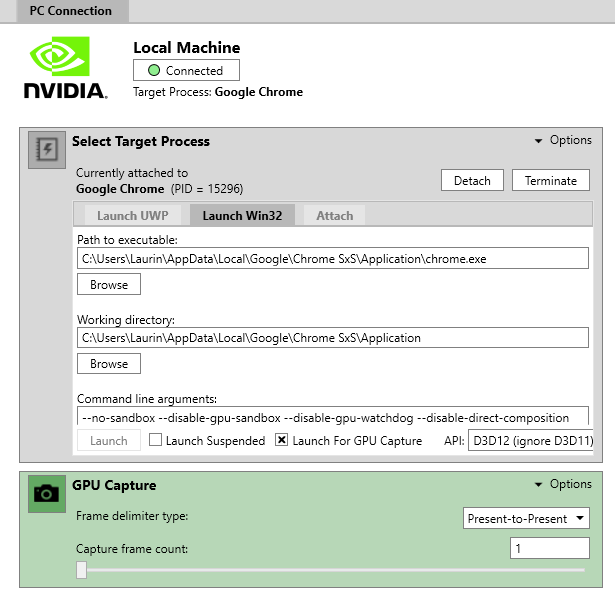
\includegraphics[width=\textwidth]{images/pix_options.png}
    \caption{Übersicht der Optionen zum Starten von \textit{Google Chrome Canary} in \textit{Microsoft PIX on Windows} \cite{microsoft:pix}. Bildschirmaufnahme durch Verfasser.}
    \label{fig:pix_options}
\end{figure}

\begin{figure}
    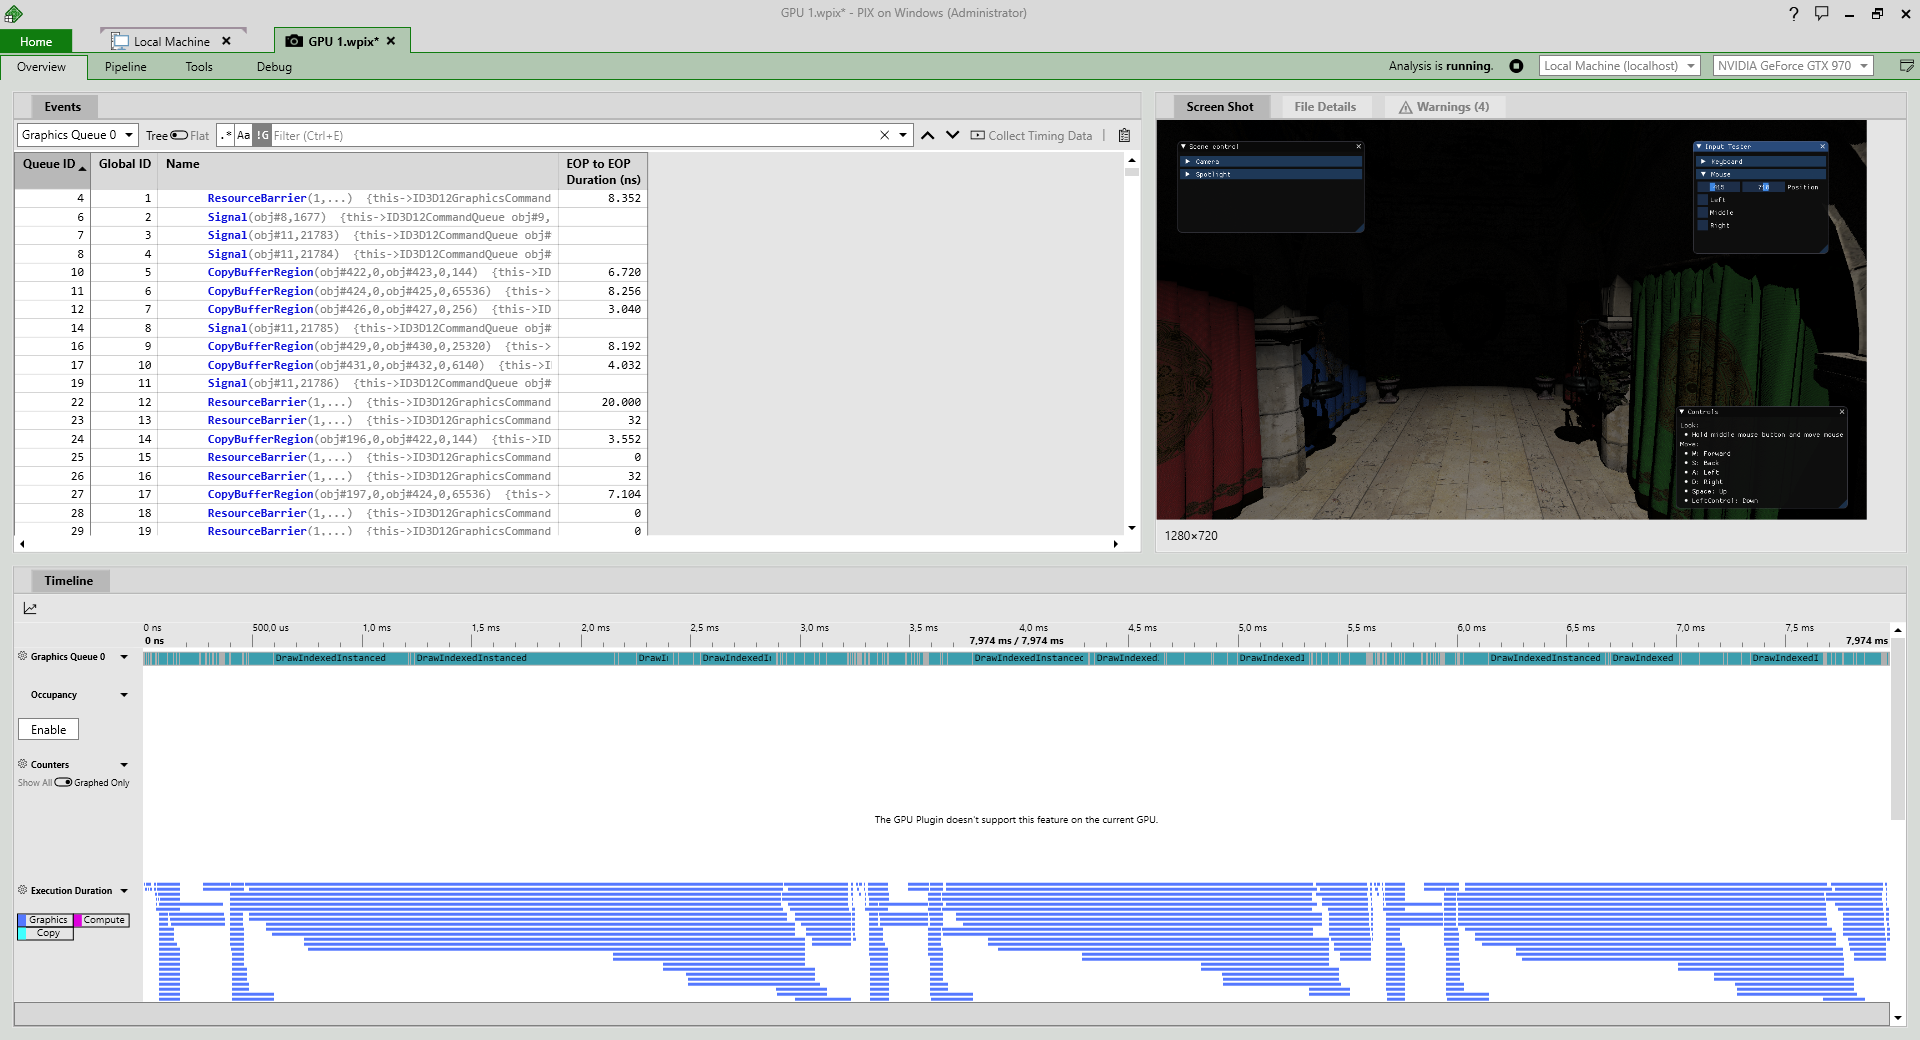
\includegraphics[width=\textwidth]{images/pix_overview.png}
    \caption{Anzeige nach der Erfassung eines Einzelbildes in \textit{Microsoft PIX on Windows} \cite{microsoft:pix}. Bildschirmaufnahme durch Verfasser.}
    \label{fig:pix_overview}
\end{figure}


%---
\chapter{Evaluierung}
\label{cha:evaluation}


%---
\chapter{Zusammenfassung und Ausblick}
\label{cha:zusammenfassung}

\section{Erreichte Ergebnisse}
\label{sec:ergebnisse}


\section{Ausblick}
\label{sec:ausblick}

\subsection{Erweiterbarkeit der Ergebnisse}
\label{sub:erweiterbarkeit}

\subsection{Übertragbarkeit der Ergebnisse}
\label{sub:uebertragbarkeit}


%-----------------------------------------------------------------------
\addcontentsline{toc}{chapter}{Referenzen}
\printbibliography[title={Referenzen}]

\appendix

%---
\chapter{Anhang A}
\label{appendix:a}
Dies ist der Quellcode zu der in Abbildung \ref{fig:spider_example_sponza} gezeigten Beispielanwendung. Die Anwendung lädt dabei das relativ komplexe 3D-Modell \textbf{Sponza} \cite{sponza} aus einer glTF-Datei \cite{khronos:gltf}, lässt den/die Anwender*in sich mit Hilfe einer steuerbaren Kamera im Raum bewegen und durch das UserInterface verschiedene Parameter der Szene verändern.
\begin{lstlisting}[language=C, label={lst:full_example}, caption={Kompletter C99-Quellcode zur Erstellung einer interaktiven 3D-Szene mit der \textbf{spider}-Engine}]
#include "spider/spider.h"

static SPLightID spot_light_id;
static uint32_t last_mouse_pos_x = 0;
static uint32_t last_mouse_pos_y = 0;
static const uint32_t surface_width = 1280;
static const uint32_t surface_height = 720;
static vec3 cam_rot = {0.0f, 0.0f, 0.0f};
static vec4 forward = {0.0f, 0.0f, 1.0f, 0.0f};
static float sensitivity = 2.0f;
static float vertical_limit = 0.01f;

void init(void) {
    // Lights have to be created before materials right now 
    const vec3 light_pos = {0.0f, 5.0f, 0.5f};
    const vec3 light_look_at = {2.0f, 0.0f, 0.0f};
    vec3 light_direction = {-1.0, -1.0f, 0.2f};
    // (float*) cast to prevent compiler warning 'incompatible-pointer-types-discards-qualifiers'
    // cglm takes no const pointers as arguments, even if it doesn't mutate the vectors
    glm_vec3_sub((float*)light_look_at, (float*)light_pos, light_direction);
    glm_vec3_normalize(light_direction);

    spot_light_id = spCreateSpotLight(&(SPSpotLightDesc){
            .pos = {light_pos[0], light_pos[1], light_pos[2]},
            .range = 40.0f,
            .color = {.r = 255, .g = 255, .b = 255},
            .dir = {light_direction[0], light_direction[1], light_direction[2]},
            .fov = glm_rad(70.0f),
            .power = 20.0f,
            .shadow_casting = &(SPLightShadowCastDesc){
                .shadow_map_size = 2048,
            },
        }
    );
    SP_ASSERT(spot_light_id.id != SP_INVALID_ID);

    /*SPSceneNodeID sponza_node_id = */spLoadGltf("assets/gltf/Sponza/Sponza.gltf");
}

bool update(float delta_time_s) {
    static bool show_controls = true;
    igBegin("Controls", &show_controls, ImGuiWindowFlags_None);
        igText("Look:");
            igBulletText("Hold right mouse button and move mouse");
        igText("Move:");
            igBulletText("W: Forward");
            igBulletText("S: Back");
            igBulletText("A: Left");
            igBulletText("D: Right");
            igBulletText("Space: Up");
            igBulletText("LeftControl: Down");
    igEnd();

    static bool scene_control = true;
    igBegin("Scene control", &scene_control, ImGuiWindowFlags_None);
    
    SPCamera* cam = spGetActiveCamera();
    glm_vec4_normalize(forward);

    if(cam) {
        if(spGetMouseButtonPressed(SPMouseButton_Right)) {
            vec2 relative_delta = {
                ((float)spGetMousePositionX() - (float)last_mouse_pos_x) / (float) surface_width,
                ((float)spGetMousePositionY() - (float)last_mouse_pos_y) / (float) surface_height
            };
            float rotation_speed = sensitivity * M_PI;
            cam_rot[1] -= rotation_speed * relative_delta[0]; // horizontal
            cam_rot[0] += rotation_speed * relative_delta[1]; // vertical
            cam_rot[0] = glm_clamp(cam_rot[0], (-M_PI * 0.5f) + vertical_limit, (M_PI * 0.5f) - vertical_limit);
        }
        memcpy(forward, (vec4){0.0f, 0.0f, 1.0f, 0.0f}, sizeof(vec4));
        mat4 rot = GLM_MAT4_IDENTITY_INIT;
        glm_euler_zyx(cam_rot, rot);
        glm_mat4_mulv(rot, forward, forward);

        cam->dir[0] = forward[0];
        cam->dir[1] = forward[1];
        cam->dir[2] = forward[2];
        vec3 sideward = {
            -forward[2],
            0.0f,
            forward[0],
        };
        glm_vec3_normalize(sideward);
        const float walk_speed = 2.0f;
        const float forward_movement = walk_speed * delta_time_s * (-1.0f * spGetKeyPressed(SPKey_S) + spGetKeyPressed(SPKey_W));
        const float sideward_movement = walk_speed * delta_time_s * (-1.0f * spGetKeyPressed(SPKey_A) + spGetKeyPressed(SPKey_D));
        const float upward_movement = walk_speed * delta_time_s * (-1.0f * spGetKeyPressed(SPKey_ControlLeft) + spGetKeyPressed(SPKey_Space));
        cam->pos[0] += forward[0] * forward_movement + sideward[0] * sideward_movement;
        cam->pos[1] += forward[1] * forward_movement + upward_movement;
        cam->pos[2] += forward[2] * forward_movement + sideward[2] * sideward_movement;
        
        if(igCollapsingHeaderTreeNodeFlags("Camera", ImGuiTreeNodeFlags_None)) {
            igSliderFloat("Look sensitivity##cam", &sensitivity, 0.0f, 5.0f, "%.1f", 1.0f);
            igSliderFloat("Vertical look limit##cam", &vertical_limit, 0.0f, M_PI * 0.5f, "%.2f", 1.0f);
            igSliderFloat3("Position##cam", (float*)&cam->pos, -10.0f, 10.0f, "%.2f", 1.0f);
            igSliderFloat3("Rotation (Rad)##cam", (float*)&cam_rot, -M_PI, M_PI, "%.2f", 1.0f);
            igSliderFloat("Vertical field of view (Rad)##cam", &cam->fovy, 0.01f, M_PI, "%.2f", 1.0f);
        }
    }

    last_mouse_pos_x = spGetMousePositionX();
    last_mouse_pos_y = spGetMousePositionY();
    
    SPLight* spot_light = spGetLight(spot_light_id);
    if(spot_light) {
        if(igCollapsingHeaderTreeNodeFlags("Spotlight", ImGuiTreeNodeFlags_None)) {
            igSliderFloat3("Position##light", (float*)&spot_light->pos, -50.0f, 50.0f, "%.1f", 1.0f);
            igSliderFloat("Field of view##light", &spot_light->fov, 0.0f, M_PI, "%.2f", 1.0f);
            igSliderFloat("Power##light", &spot_light->power, 0.0f, 1000.0f, "%.0f", 1.0f);
            igSliderFloat("Range##light", &spot_light->range, 0.0f, 1000.0f, "%.0f", 1.0f);
        }
    }
    igEnd();

    // return false if you want to quit
    return true;
}

int main() {
    spInit(&(SPInitDesc){
        .surface_size = {
            .width = surface_width,
            .height = surface_height
        },
        .update_func = update,
        .camera = {
            .pos = {0.0f, 2.0f, 0.0f},
            .dir = {0.0f, 0.0f, 1.0f},
            .look_at = {0.0f, 0.0f, 0.0f},
            .mode = SPCameraMode_Direction,
            .fovy = glm_rad(60.0f),
            .aspect = (float)surface_width / (float) surface_height,
            .near = 0.1f,
        },
        .pools.capacities = {
            .meshes = 128,
            .materials = 64,
            .render_meshes = 256,
            .lights = 1,
            .scene_nodes = 1024,
        },
        .show_stats = true,
    });

    init();

    spStart();
    return 0;
}
\end{lstlisting}

%---
\chapter{Anhang B}
\label{appendix:b}

\begin{lstlisting}[language=glsl, label={lst:fragment_shader}, caption={Kompletter GLSL-Code des Fragment-Shaders der in der \textbf{spider}-Engine für das \ac{PBR} benutzt wird}]
#version 450
#extension GL_ARB_separate_shader_objects : enable
#extension  GL_EXT_samplerless_texture_functions : enable

layout(set = 0, binding = 1) uniform Camera {
    mat4 view;
    mat4 proj;
    vec3 pos;
} cam;

layout(set = 0, binding = 2) uniform Light {
    mat4 view;
    mat4 proj;
    vec4 pos3_range1;
    vec4 color3_type1; // type: 0 directional, 1 spot, 2 point
    vec4 dir3_fov1; // dir: for spot & dir, fov: for spot
    vec4 area2_power1_padding1; // area: for dir
} light;  // TODO: support more than 1 light

layout(set = 2, binding = 0) uniform texture2D albedo_tex;
layout(set = 2, binding = 1) uniform sampler albedo_sampler;
layout(set = 2, binding = 2) uniform texture2D normal_tex;
layout(set = 2, binding = 3) uniform sampler normal_sampler;
layout(set = 2, binding = 4) uniform texture2D ao_roughness_metallic_tex;
layout(set = 2, binding = 5) uniform sampler arm_sampler;
layout(set = 2, binding = 6) uniform texture2D shadow_map;
layout(set = 2, binding = 7) uniform sampler shadow_sampler;


layout(location = 0) in vec3 fragPosWorld;
layout(location = 1) in vec2 fragTexCoords;
layout(location = 2) in vec3 fragNormal;
layout(location = 3) in vec3 fragTangent;

layout(location = 0) out vec4 outColor;

const float PI = 3.14159265359;
const float gamma = 2.2;

const int sampleSize = 1;
const float scale = 1.5;

float getLightDepthOnPosSingle(vec2 coords_shadow_map) {
    return texture( sampler2D( shadow_map, shadow_sampler ), coords_shadow_map.xy ).r;
}

float getLightDepthOnPosSampled(vec2 coords_shadow_map) {
    float value = 0.0;
    ivec2 texDim = textureSize(shadow_map, 0);
    float dx = scale * 1.0 / float(texDim.x);
    float dy = scale * 1.0 / float(texDim.y);
    int count = 0;
    for(int y = -sampleSize; y <= sampleSize; ++y) {
        for(int x = -sampleSize; x <= sampleSize; ++x) {
            value += getLightDepthOnPosSingle(coords_shadow_map + vec2(x * dx, y * dy));
            count++;
        }
    }
    return value / count;
}

float DistributionGGX(vec3 N, vec3 H, float roughness) {
    float a      = roughness*roughness;
    float a2     = a*a;
    float NdotH  = max(dot(N, H), 0.0);
    float NdotH2 = NdotH*NdotH;
	
    float num   = a2;
    float denom = (NdotH2 * (a2 - 1.0) + 1.0);
    denom = PI * denom * denom;
	
    return num / denom;
}

float GeometrySchlickGGX(float NdotV, float roughness) {
    float r = (roughness + 1.0);
    float k = (r*r) / 8.0;

    float num   = NdotV;
    float denom = NdotV * (1.0 - k) + k;
	
    return num / denom;
}
float GeometrySmith(vec3 N, vec3 V, vec3 L, float roughness) {
    float NdotV = max(dot(N, V), 0.0);
    float NdotL = max(dot(N, L), 0.0);
    float ggx2  = GeometrySchlickGGX(NdotV, roughness);
    float ggx1  = GeometrySchlickGGX(NdotL, roughness);
	
    return ggx1 * ggx2;
}

vec3 fresnelSchlick(float cosTheta, vec3 F0) {
    return F0 + (1.0 - F0) * pow(1.0 - cosTheta, 5.0);
}

void main() {
    const vec4 albedo_all = texture(sampler2D(albedo_tex, albedo_sampler), fragTexCoords).rgba;
    const vec3 albedo = albedo_all.rgb;
    const float alpha = albedo_all.a;
    if(alpha == 0.0) {
        discard;
    }
    vec3 tangent_space_normal = normalize(texture(sampler2D(normal_tex, normal_sampler), fragTexCoords).xyz * vec3(2.0, 2.0, 1.0) - vec3(1.0, 1.0, 0.0));
    const vec3 ao_roughness_metallic = texture(sampler2D(ao_roughness_metallic_tex, arm_sampler), fragTexCoords).rgb;
    const float ao          = ao_roughness_metallic.r;
    const float roughness   = ao_roughness_metallic.g;
    const float metallic    = ao_roughness_metallic.b;

    vec3 Normal = normalize(fragNormal);
    vec3 Tangent = normalize(fragTangent);
    // enforce orthogonality
    Tangent = normalize(Tangent - dot(Tangent, Normal) * Normal);
    const vec3 Bitangent = cross(Tangent, Normal);
    mat3 TBN = mat3(Tangent, Bitangent, Normal);
    vec3 normal = normalize(TBN * tangent_space_normal);

    vec3 N = normalize(normal);
    vec3 V = normalize(cam.pos - fragPosWorld);
    vec3 F0 = vec3(0.04); 
    F0 = mix(F0, albedo, metallic);
	           
    // reflectance equation
    vec3 Lo = vec3(0.0);
    vec3 light_pos = light.pos3_range1.xyz;
    float distance    = length(light_pos - fragPosWorld);
    vec3 L = normalize(light_pos - fragPosWorld);
    float light_fov = 1.0 - (light.dir3_fov1.w / 3.14);
    float attenuation = light.area2_power1_padding1.z * (light_fov * light_fov);
    attenuation *= max(1.0 - distance / light.pos3_range1.w, 0.0);
    
    // For spot lights
    if(light.color3_type1.w == 1.0) {
        const float light_angle_rad = acos(dot(light.dir3_fov1.xyz, -L));
        attenuation *= pow(max(light.dir3_fov1.w * 0.5 - light_angle_rad, 0.0) / 3.14, 1.0 - (light_fov * light_fov));
    }
    // Shadow calculation
    const vec4 pos_shadow_map = light.proj * light.view * vec4(fragPosWorld, 1.0);
    vec4 pos_in_light_clip_space = pos_shadow_map / pos_shadow_map.w;
    pos_in_light_clip_space.xy = pos_in_light_clip_space.xy * 0.5 + 0.5; // [-1,1] to [0,1]
    pos_in_light_clip_space.y = 1.0 - pos_in_light_clip_space.y; // bottom-up to top-down
    // [0, 0] of pos_in_light_clip_space.xy should now be the top left corner and [1, 1] the bottom right --> texture space

    const float depth_bias = 0.00001; // Depth bias is not yet implemented in Chromium/dawn, so we have to "fake" it in the shader
    if(attenuation > 0.0 && pos_in_light_clip_space.z > 0.0 && pos_in_light_clip_space.z < 1.0) {
        const float light_depth_on_pos = getLightDepthOnPosSampled(pos_in_light_clip_space.xy);
        if(pos_in_light_clip_space.w > 0.0 && light_depth_on_pos - depth_bias > pos_in_light_clip_space.z) {
            attenuation = 0.0;
        }
    }
    if(attenuation > 0.0) {
        // calculate per-light radiance
        vec3 H = normalize(V + L);
        vec3 radiance     = light.color3_type1.rgb * attenuation;
        
        // cook-torrance brdf
        float NDF = DistributionGGX(N, H, roughness);
        float G   = GeometrySmith(N, V, L, roughness);
        vec3 F    = fresnelSchlick(max(dot(H, V), 0.0), F0);
        
        vec3 kS = F;
        vec3 kD = vec3(1.0) - kS;
        kD *= 1.0 - metallic;
        
        vec3 numerator    = NDF * G * F;
        float denominator = 4.0 * max(dot(N, V), 0.0) * max(dot(N, L), 0.0);
        vec3 specular     = numerator / max(denominator, 0.001);  
            
        // add to outgoing radiance Lo
        float NdotL = max(dot(N, L), 0.0);                
        Lo += (kD * albedo / PI + specular) * radiance * NdotL;
    }
  
    vec3 ambient = vec3(0.04) * albedo * ao;
    vec3 color = ambient + Lo;
	
    color = color / (color + vec3(1.0));
    color = pow(color, vec3(1.0/gamma));  
   
    outColor = vec4(color, alpha);
}
\end{lstlisting}

\chapter{Anhang C}
\label{appendix:c}
\begin{lstlisting}[language=glsl, label={lst:vert_full}, caption={Kompletter GLSL-Code des Vertex-Shaders für das Minimalbeispiel aus Kapitel \ref{cha:example}}]
#version 450

layout(set = 0, binding = 0) uniform Common {
    mat4 view;
    mat4 proj;
};

layout(set = 1, binding = 0) uniform Dynamic {
    mat4 model;
};

layout (location = 0) in vec3 inPos;
layout (location = 1) in vec3 inColor;

layout (location = 0) out vec3 outColor;

void main() {
    vec4 pos = proj * view * model * vec4(inPos, 1.0);
    outColor = inColor;
    gl_Position = pos;
}
\end{lstlisting}
\begin{lstlisting}[language=glsl, label={lst:fragment_shader}, caption={Kompletter GLSL-Code des Fragment-Shaders für das Minimalbeispiel aus Kapitel \ref{cha:example}}]
#version 450

layout (location = 0) in vec3 inColor;

layout (location = 0) out vec4 outFragColor;

void main() {
    outFragColor = vec4(inColor, 1.0);
}
\end{lstlisting}
\begin{lstlisting}[language=HTML, label={lst:html_full}, caption={Kompletter HTML-Quellcode für das Minimalbeispiel aus Kapitel \ref{cha:example}}]
<html>
<body>
    <canvas id="canvas" width="800" height="600"></canvas>
    <script src="webgpu.js"></script>
</body>
</html>
\end{lstlisting}

\begin{lstlisting}[language=JavaScript, label={lst:js_full}, caption={Kompletter JavaScript-Quellcode für das Minimalbeispiel aus Kapitel \ref{cha:example}}]
async function loadShader(shaderPath) {
   return await fetch(new Request(shaderPath), { method: 'GET', mode: 'cors' }).then((res) =>
        res.arrayBuffer().then((arr) => new Uint32Array(arr))
    );
}

function initBuffer(data, usage, device, queue) {
    const use_write_buffer = true;
    if(use_write_buffer && queue["writeBuffer"] !== undefined){
        var buffer = device.createBuffer({
            size: data.byteLength,
            usage: usage | GPUBufferUsage.COPY_DST
        });
        queue.writeBuffer(buffer, 0, data.buffer);
        return buffer;
    }
    else {
        var [buffer, buffer_data] = device.createBufferMapped({
            size: data.byteLength,
            usage: usage
        });
        var writeArray = data instanceof Uint16Array ? new Uint16Array(buffer_data) : new Float32Array(buffer_data);
        writeArray.set(data);
        buffer.unmap();
        return buffer;
    }
}

async function start() {
    var gpu = navigator.gpu;
    var adapter = await gpu.requestAdapter({powerPreference: "high-performance"});
    var device = await adapter.requestDevice();
    var queue = device.defaultQueue;
    // Vertex Data (4 vertices with each 3 float for position and 3 float for color)
    const vertex_data = new Float32Array([
    //     x,    y,   z,      r,   g,   b
        -1.0,  1.0, 0.5,    1.0, 0.0, 0.0,
         1.0,  1.0, 0.5,    0.0, 1.0, 0.0,
        -1.0, -1.0, 0.5,    0.0, 0.0, 1.0,
         1.0, -1.0, 0.5,    1.0, 1.0, 1.0,
    ]);

    var vertex_buffer = initBuffer(vertex_data, GPUBufferUsage.VERTEX, device, queue);

    // Index data (2 triangles with each 3 indices)
    const index_data = new Uint16Array([
        0, 1, 2, 
        2, 1, 3
    ]);

    var index_buffer = initBuffer(index_data, GPUBufferUsage.INDEX, device, queue);

    var texture = device.createTexture({
        size: {
            width: 1024,
            height: 1024,
            depth: 1
        },
        mipLevelCount: 1,
        sampleCount: 1,
        dimension: '2d',
        format: 'rgba8unorm',
        usage: GPUTextureUsage.SAMPLED | GPUTextureUsage.COPY_DST
    });
    console.log(texture);

    var texture_data = new Uint32Array(1024 * 1024);
    texture_data.fill(0x00FF00FF); // 0 red, 255 blue, 0 green, 255 alpha

    var texture_copy_view = {
        texture: texture,
        mipLevel: 0,
        origin: {
            x: 0,
            y: 0,
            z: 0
        }
    };
    
    var data_layout = {
        offset: 0,
        bytesPerRow: 1024 * 4,
        rowsPerImage: 1024
    };

    var copy_size = {
        width: 0,
        height: 0,
        depth: 0
    };
    if(queue["writeTexture"] !== undefined) {
        queue.writeTexture(texture_copy_view, texture_data, data_layout, copy_size);
    }
    else {
        console.log("writeTexture not implemented");
    }

    // bgle = BindGroupLayoutEntry
    // bgl = BindGroupLayout

    var bgle_view_proj = {
        binding: 0,
        visibility: GPUShaderStage.VERTEX,
        type: 'uniform-buffer',
        hasDynamicOffset: false
    };
    
    var bgl_common = device.createBindGroupLayout({
        entries: [
            bgle_view_proj
        ]
    });

    var bgle_model = {
        binding: 0,
        visibility: GPUShaderStage.VERTEX,
        type: 'uniform-buffer',
        hasDynamicOffset: false
    };

    var bgl_dynamic = device.createBindGroupLayout({
        entries: [
            bgle_model
        ]
    });

    var pipeline_layout = device.createPipelineLayout({
        bindGroupLayouts: [
            bgl_common,
            bgl_dynamic
        ]
    });

    var canvas = document.getElementById('canvas');
    var canvas_context = canvas.getContext('gpupresent');
    const canvas_format = await canvas_context.getSwapChainPreferredFormat(device);
    var swap_chain = canvas_context.configureSwapChain({
        device: device,
        format: canvas_format,
        usage: GPUTextureUsage.OUTPUT_ATTACHMENT
    });

    const vertex_shader_code_spirv = await loadShader('simple.vert.spv');
    const frag_shader_code_spirv = await loadShader('simple.frag.spv');

    var render_pipeline = device.createRenderPipeline({
        layout: pipeline_layout,
        vertexState: {
            indexFormat: 'uint16',
            vertexBuffers: [
                {
                    arrayStride: 24, // 24 bytes per vertex
                    stepMode: 'vertex',
                    attributes: [
                        { // pos attribute
                            format: 'float3',
                            offset: 0,
                            shaderLocation: 0
                        },
                        { // color attribute
                            format: 'float3',
                            offset: 12, // offset in bytes
                            shaderLocation: 1
                        }
                    ]
                }
            ]
        },
        vertexStage: {
            module: device.createShaderModule({
                code: vertex_shader_code_spirv
            }),
            entryPoint: 'main'
        },
        primitiveTopology: 'triangle-list',
        rasterizationState: {
            frontFace: 'cw', // clock wise
            cullMode: 'none', // don't cull faces
        },
        fragmentStage: {
            module: device.createShaderModule({
                code: frag_shader_code_spirv
            }),
            entryPoint: 'main'
        },
        depthStencilState: {
            format: 'depth32float',
            depthWriteEnabled: true,
            depthCompare: 'greater'
        },
        colorStates: [
            {
                format: canvas_format,
                alphaBlend: { 
                    srcFactor: 'one', 
                    dstFactor: 'zero', 
                    operation: 'add'
                },
                colorBlend: { 
                    srcFactor: 'one', 
                    dstFactor: 'zero', 
                    operation: 'add'
                },
                writeMask: GPUColorWrite.ALL
            }
        ]
    });

    var common_data = new Float32Array([
        // view matrix
        1.0, 0.0, 0.0, 0.0,
        0.0, 1.0, 0.0, 0.0,
        0.0, 0.0, 1.0, 0.0,
        0.0, 0.0, 0.0, 1.0,
        // proj matrix
        1.0, 0.0, 0.0, 0.0,
        0.0, 1.0, 0.0, 0.0,
        0.0, 0.0, 1.0, 0.0,
        0.0, 0.0, 0.0, 1.0,
    ]);

    var common_buffer = initBuffer(common_data, GPUBufferUsage.UNIFORM, device, queue);

    var bind_group_common = device.createBindGroup({
        layout: bgl_common,
        entries: [
            {
                binding: 0,
                resource: {
                    buffer: common_buffer,
                    offset: 0,
                    size: common_data.byteLength
                }
            }
        ]
    });

    var model_data = new Float32Array([
        // model matrix (translate 2 units in Z direction)
        1.0, 0.0, 0.0, 0.0,
        0.0, 1.0, 0.0, 0.0,
        0.0, 0.0, 1.0, 0.0,
        0.0, 0.0, 0.0, 1.0
    ]);

    var dynamic_buffer = initBuffer(model_data, GPUBufferUsage.UNIFORM, device, queue);

    var bind_group_dynamic = device.createBindGroup({
        layout: bgl_dynamic,
        entries: [
            {
                binding: 0,
                resource: {
                    buffer: dynamic_buffer,
                    offset: 0,
                    size: model_data.byteLength
                }
            }
        ]
    });
    
    render(device, swap_chain, queue, canvas, render_pipeline, vertex_buffer, index_buffer, bind_group_common, bind_group_dynamic, index_data);

}

function render(device, swap_chain, queue, canvas, render_pipeline, vertex_buffer, index_buffer, bind_group_common, bind_group_dynamic, index_data) {
    var color_texture = swap_chain.getCurrentTexture();
    var depth_texture = device.createTexture({
        size: {
            width: canvas.width,
            height: canvas.height,
            depth: 1
        },
        mipLevelCount: 1,
        sampleCount: 1,
        dimension: '2d',
        format: 'depth32float',
        usage: GPUTextureUsage.OUTPUT_ATTACHMENT
    });

    var command_enc = device.createCommandEncoder();
    var render_pass = command_enc.beginRenderPass({
        colorAttachments: [
            {
                attachment: color_texture.createView(),
                loadValue: {r: 0.3, g: 0.0, b: 0.2, a: 1.0}, // clear to dark purple
                storeOp: 'store'
            }
        ],
        depthStencilAttachment: {
            attachment: depth_texture.createView(),
            depthLoadValue: 0.0,
            depthStoreOp: 'store',
            depthReadOnly: false,
            stencilLoadValue: 0,
            stencilStoreOp: 'store',
            stencilReadOnly: true
        },
    });

    render_pass.setPipeline(render_pipeline);
    render_pass.setVertexBuffer(0, vertex_buffer);
    render_pass.setIndexBuffer(index_buffer);
    render_pass.setBindGroup(0, bind_group_common);
    render_pass.setBindGroup(1, bind_group_dynamic);
    render_pass.drawIndexed(index_data.length);
    render_pass.endPass();

    var command_buffer = command_enc.finish();
    queue.submit([command_buffer]);

    requestAnimationFrame(function() {
        render(device, swap_chain, queue, canvas, render_pipeline, vertex_buffer, index_buffer, bind_group_common, bind_group_dynamic, index_data);
    });
}

start();
\end{lstlisting}

\end{document}